\documentclass{article}

%-- My Definitions
\usepackage{mydefs}

%-- Math stuff
\usepackage{mathtools, amsfonts, amsthm, amssymb}
%-- Physics and Chemistry stuff
\usepackage[version=4]{mhchem}
\usepackage{braket}
\usepackage{siunitx}
\sisetup{
    input-digits = 0123456789\pi,
    separate-uncertainty,
    table-align-uncertainty,
    table-number-alignment = center
}

%to compile Feynman diagrams: uncomment these
%can take a lot of compile time, set the compiler to LuaLaTex
%\usepackage[compat=1.1.0]{tikz-feynman}
%\usepackage{tikz}

%-- Computer science stuffError
\usepackage{algorithm, algpseudocode}
%\usepackage{minted}
%-- Plotting
%\usepackage{graphicx}

%-- Tables and enumerations
\usepackage{enumerate}
\usepackage{booktabs, multirow}
\usepackage{caption, subcaption}

%-- Bibliography
\usepackage{csquotes}
\usepackage[
  backend=biber,
  style=numeric,
  citestyle=numeric,
  sorting=none
]{biblatex}
\addbibresource{bibliography.bib}

%-- Numbering
\numberwithin{equation}{section}
\numberwithin{algorithm}{section}
\counterwithin{figure}{section}
\counterwithin{table}{section}


%-- General Formatting
\usepackage[top=20mm,bottom=20mm,left=25mm,right=25mm]{geometry}
\usepackage[english]{babel}
\selectlanguage{english}
\usepackage[colorlinks=true, allcolors=blue]{hyperref}
\usepackage{fancyhdr}
\usepackage{parskip}
\usepackage{csquotes}
%\setlength{\parindent}{0pt}
%\setlength{\parskip}{0.5\baselineskip}

%-----> Document begins here <-----
\begin{document}

% -- Title page

\title{Template}
\author{Author}
\date{\today}
\maketitle

\clearpage

\begin{abstract}
This report presents the methods, results, and discussion of the internship work.
The focus is on the relevant physics background, experimental setup, and error
analysis. Results are compared to theoretical expectations and summarized in the
conclusion.
\end{abstract}
\clearpage

% -- Table of contents
\setcounter{tocdepth}{2}
\tableofcontents

\clearpage


\section{Introduction}
Briefly explain the motivation and objectives of the internship project.

\section{Theory}




\subsection[Origin of the HI-Line]{Origin of the \ce{H_I}-Line}

\subsection{Angular resolution of the SRT}\label{sec:ang_res}
Using the equation relating the effective area $A_e$ and the wavelength $\lambda$ \cite[p. 149 (7.11)]{wilson}
\begin{equation}
    A_e \Omega_A = \lambda^2
\end{equation}
Using the definitions of the effective area and the geometric area
\begin{equation}
    A_e = \eta A_g \qquad A_g = \pi \left( \frac{d}{2} \right) \label{eq:A_e}
\end{equation}
we can then solve for the effective antenna area.
\begin{equation}
    \Omega_A = \frac{\lambda^2}{A_g \eta} \label{eq:Omega_A}
\end{equation}
We only need to relate a solid-angle $\Omega$ to an angular resolution $\theta$ now. We define $\theta$ to be the half-angle that spans the solid-angle $\Omega$ on the unit sphere and thus arrive at the following expression.
\begin{align}
    \Omega = \int_{0}^{2\pi} d\phi \int_{0}^{\theta} d\vartheta \sin(\vartheta) \notag \\
    \Omega = 4 \pi \sin^2 \left( \frac{\theta}{2} \right) \approx \pi \theta^2 \label{eq:solid_angle}
\end{align}
By solving \eqref{eq:solid_angle} for $\theta$ and inserting \eqref{eq:Omega_A} and \eqref{eq:A_e} we get the final result.
\begin{equation}
    \theta_A = \sqrt{\frac{\Omega_A}{\pi}} = \sqrt{\frac{\lambda^2}{\frac{1}{4} \pi d^2 \eta \pi}} = \frac{2\lambda}{\pi d \sqrt{\eta}} \label{eq:half_angle}
\end{equation}

To compute the angular resolution we need the diameter of the SRT which is $d = \SI{4}{m}$ \cite[p. 4]{srt}, and the antenna efficiency which is $\eta = 0.5$ \cite[p. 2]{srt}.
Unfortunately we cannot reasonably estimate an error for the antenna efficiency $\eta$, we suspect however that the error of the antenna efficiency dominates here.
Therefore we will waive a proper error discussion here.

It is important to note that this angle is the half of the equivalent beam width, not the full width at half maximum, but this value will become useful in subsection \ref{sec:temp}.

To compute an approximation of the FWHM we can approximate the aperture as gaussian \cite[p. 2]{script} and note the following properties.
\begin{equation}
    \Omega_A \approx \int_{4\pi } d\Omega \exp{\left( -\frac{\theta^2}{2\sigma^2} \right)} \approx 4\pi \int_0^{\infty} d\theta \theta \exp{\left( -\frac{\theta^2}{2\sigma^2} \right)} = 4\pi \sigma^2
    \label{eq:gauss_integral}
\end{equation}
\begin{equation}
    \exp{\left( -\frac{(\theta_{FWHM}/2)^2}{2\sigma^2}\right)} = \frac{1}{2} \quad \implies \quad \theta_{\text{FWHM}} = 2 \sqrt{2\ln{2}} \sigma \label{eq:FWHM}
\end{equation}
using equations \eqref{eq:half_angle} - \eqref{eq:FWHM} we can then solve for $\theta_{\text{FWHM}}$
\begin{equation}
    \theta_{\text{FWHM}} = \sqrt{2\ln{2}} \, \theta_A
\end{equation}

We can then obtain the values shown in table \ref{tab:ang_res}.
\begin{table}[h]
    \centering
    \begin{tabular}{rrrr}
        \toprule
        $\theta_{\text{FWHM}}$ & Angular resolution $\theta$ & Wavelength $\lambda$ & Frequency\\
        \midrule
        \SI{3.206}{\degree} &\SI{2.723}{\degree} & \SI{21.11}{cm} & \SI{1.420}{\giga \hertz}\\
        \SI{0.455}{\degree} &\SI{0.387}{\degree} & \SI{0.30}{cm} & \SI{10.000}{\giga \hertz}\\
        \bottomrule
    \end{tabular}
    \caption{Angular resolution of the SRT at different frequencies}
    \label{tab:ang_res}
\end{table}
\subsection{Antenna, brightness and noise temperature}

\subsection{Temperature conversion}

\subsection{Expected temperature of the sun}\label{sec:temp}
If we assume that the sun is a black body near the wavelength of \SI{1.42}{\giga\hertz} we expect it to have a brightness temperature of $T_{\odot} = \SI{5778}{\kelvin}$ \cite[p. 211]{ftb}.
We have to consider however, that the half-angle size of the sun with a value of \SI{16}{\arcminute} \cite[p. 211]{ftb} is less than the angular resolution we computed in table \ref{tab:ang_res}.
Because the power measured by the telescope and the brightness temperature have a linear relationship knowing the beam filling factor $B$ will suffice.
\begin{equation}
    B = \frac{\Omega_{\odot}}{\Omega_A} = \frac{\theta_{\odot}^2}{\theta_A^2} = \SI{0.96
    }{\percent}
\end{equation}
We know that the sky itself will also contribute a temperature of $T_{\text{sky}} = \SI{2.7}{\kelvin}$ \cite[p. 4]{script}, thus we obtain at the final result.
\begin{equation}
    T_{\text{measured}} = B T_{\odot} (1-B) T_{\text{sky}} = \SI{58}{\kelvin}
\end{equation}
This result is given without error due to the same reasons as in section \ref{sec:ang_res}


\subsection{Influence of elevation angle}

\subsection{Doppler shift}

\section{Materials and Methods}

\subsection{Small Radio Telescope (SRT)}
All measurements were performed using the small radio telescope located on top of the ExWi building.
It has a parabolic dish with a diameter of \SI{4}{m} and a feedhorn antenna. This causes main and side lobes, where the shape of the main lobe can be approximated as Gaussian.

\subsubsection{Signal Processing}
\begin{figure}[H]
    \centering
    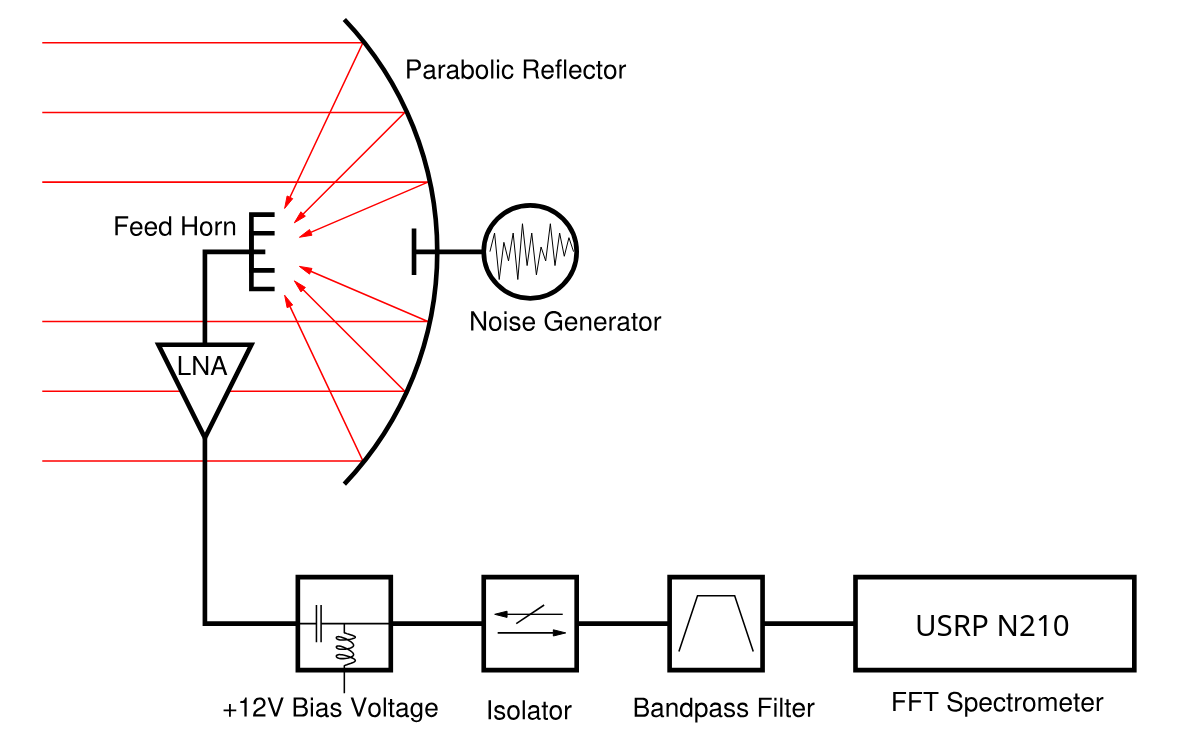
\includegraphics[width=0.6\textwidth]{assets/schematic.png}
    \caption{Schematic of the signal process. \cite[Fig. 3]{srt} hTODO: FIX THE SCHEMATIC}
    \label{fig:signal}
\end{figure}
The signal processing is shown schematically in Figure \ref{fig:signal}.
After the radiowaves are focused by the parabolic dish and received by the feedhorn antenna, they are first amplified by a low noise amplifier (LNA).
The amplified signal is then transmitted through a coaxial cable into the laboratory, where it passes through the receiver chain. This includes a bias-T that injects the supply voltage for the LNA,
a microwave isolator to prevent reflections, and a band-pass filter restricting the signal to the frequency range of \qtyrange{1.400}{1.427}{GHz}.
TODO: THE SQUARING CIRCUIT IS NOT IN THE SCHEMATIC, BUT SHOULD PROBABLY BE DESCRIBED HERE!
Finally, the filtered signal enters a digital spectrometer based on the \quote{Universal Software Defined Radio} (USRP) receiver,
where it is down-converted, digitized, and analyses using a Fast Fourier Transform (FFT). \cite[Sec. 4]{srt}

The outputs of the Fourier transform are spectral amplitude densities with units of [\si{\volt/\hertz}]. This value is proportional to the power density and its integration is proportional to the power.
This can lead to confusion if we denote axes in figures with units of Volts even though their physical interpretation should be as a value of Power.
For the rest of this report we will denote the unit of this amplitude in arbitrary units [\si{a.u.}] and the spectral amplitude density with units of [\si{a.u./\hertz}].
We will also use the symbol $P$ to denote such values to better convey the physical meaning.

\subsection{Lab View Tool}
sketch, description


\subsection{Measurement data and Code}
All data and code used in this report are available in a public repository\footnote{\url{https://github.com/SecretGmG/lab/tree/main/srt}}.

Error propagation and data fitting were performed using the publicly available module PhysicsTool\footnote{\url{https://github.com/SecretGmG/PhysicsTool}}.
\section{Measurements and Results}
\subsection{Elevation Scan}
We performed an elevation scan from the horizon \SI{10}{\degree} to the zenith \SI{90}{\degree} at different  azimuth angles.
We chose an angular step size of \SI{1}{\degree}. This step size was chosen as a compromise between measurement time and angular resolution.
For these Measurements we made sure that the sun does not cross the scan path. We performed two measurements at different times of the day.

\begin{figure}[H]
\centering
\begin{subfigure}[t]{0.45\textwidth}
    \centering
    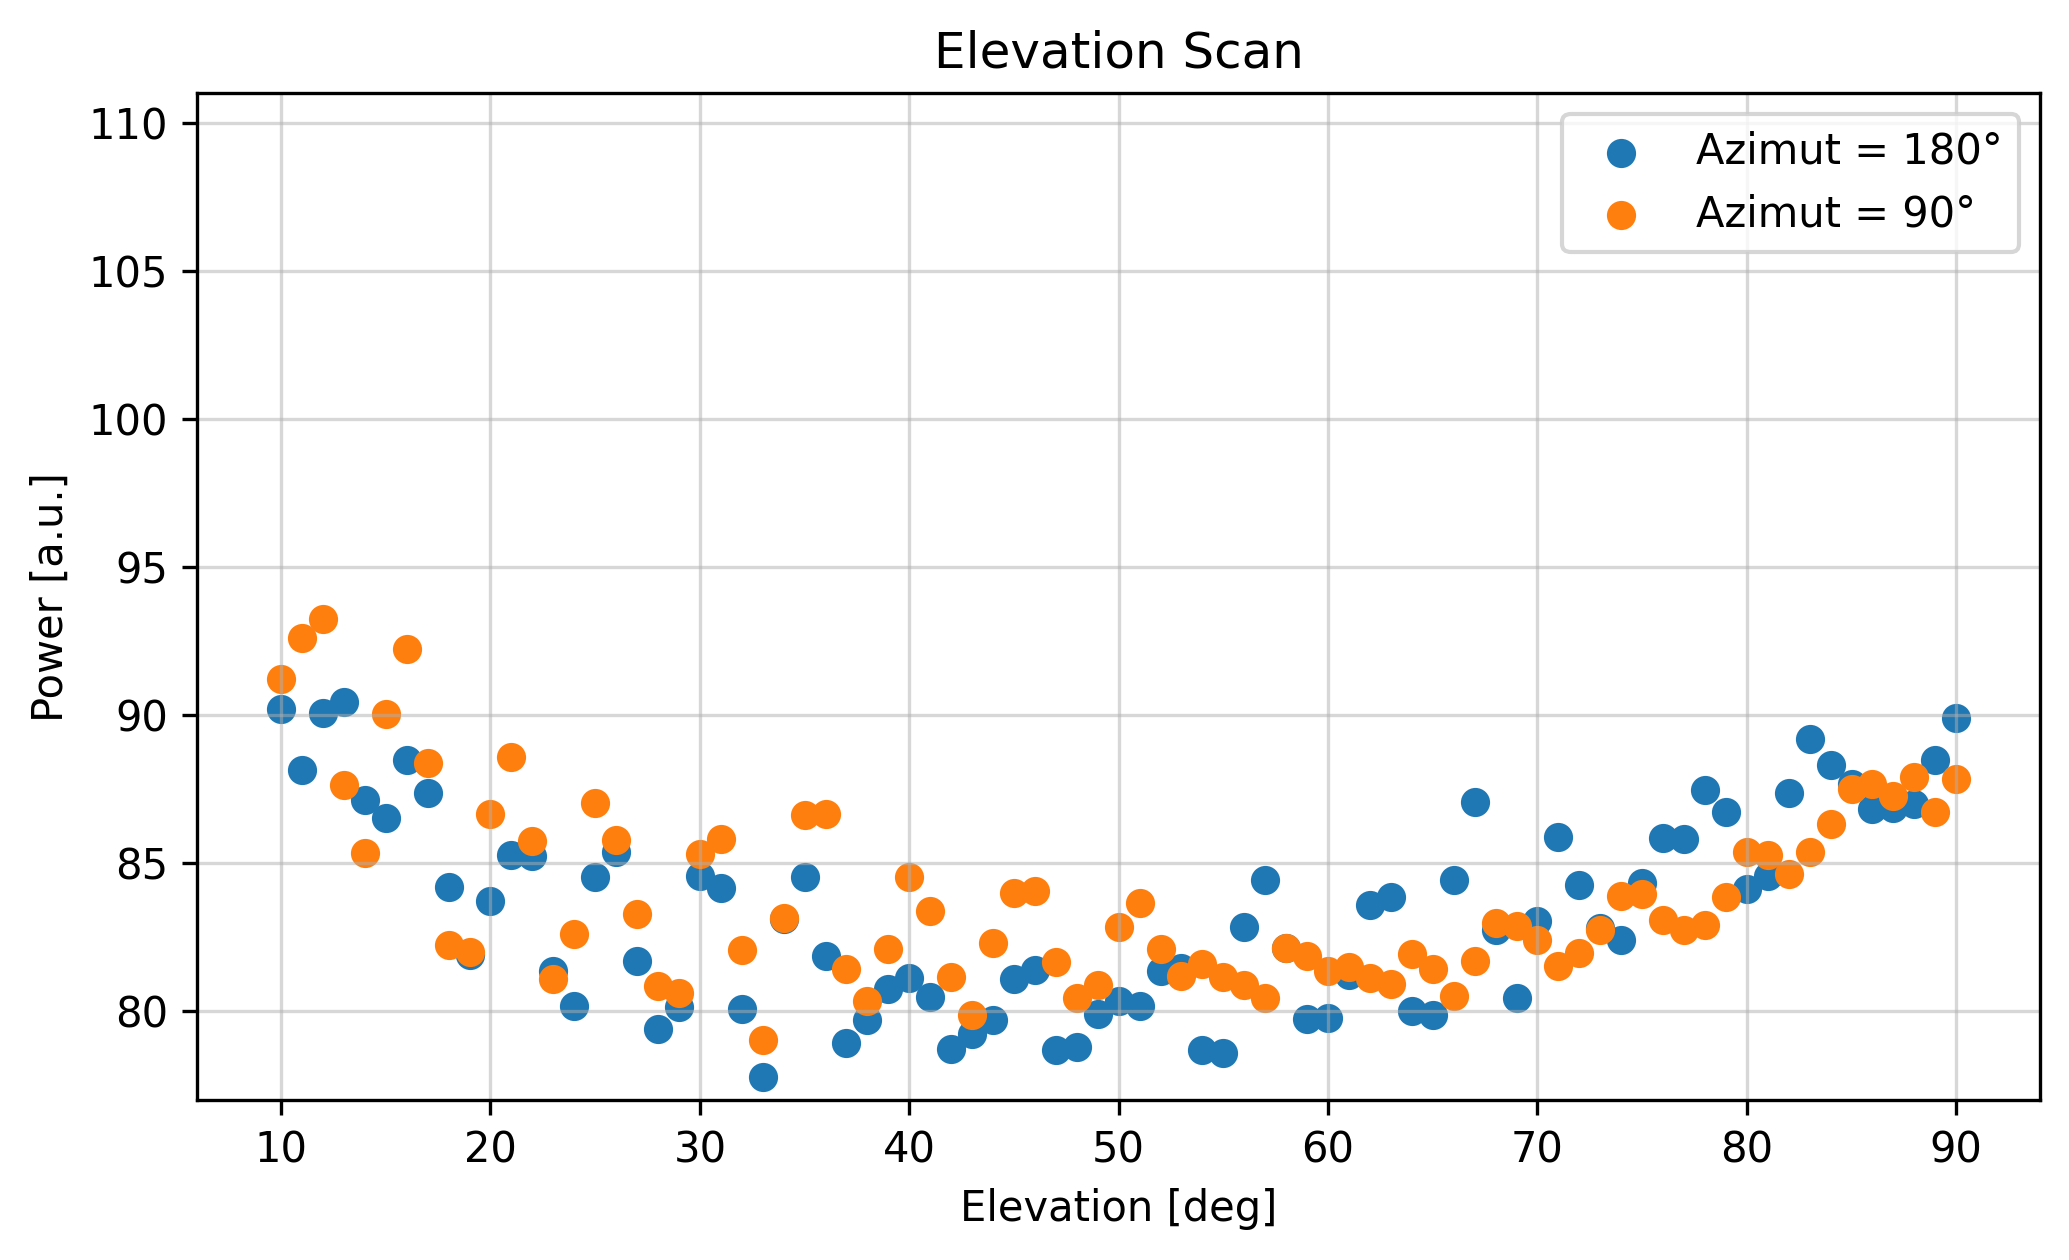
\includegraphics[width=\linewidth]{assets/elev_scan_night.png}
    \caption{Elevation Scan \texttt{01.10.2025 22:35 MESZ}}
\end{subfigure}
\begin{subfigure}[t]{0.45\textwidth}
    \centering
    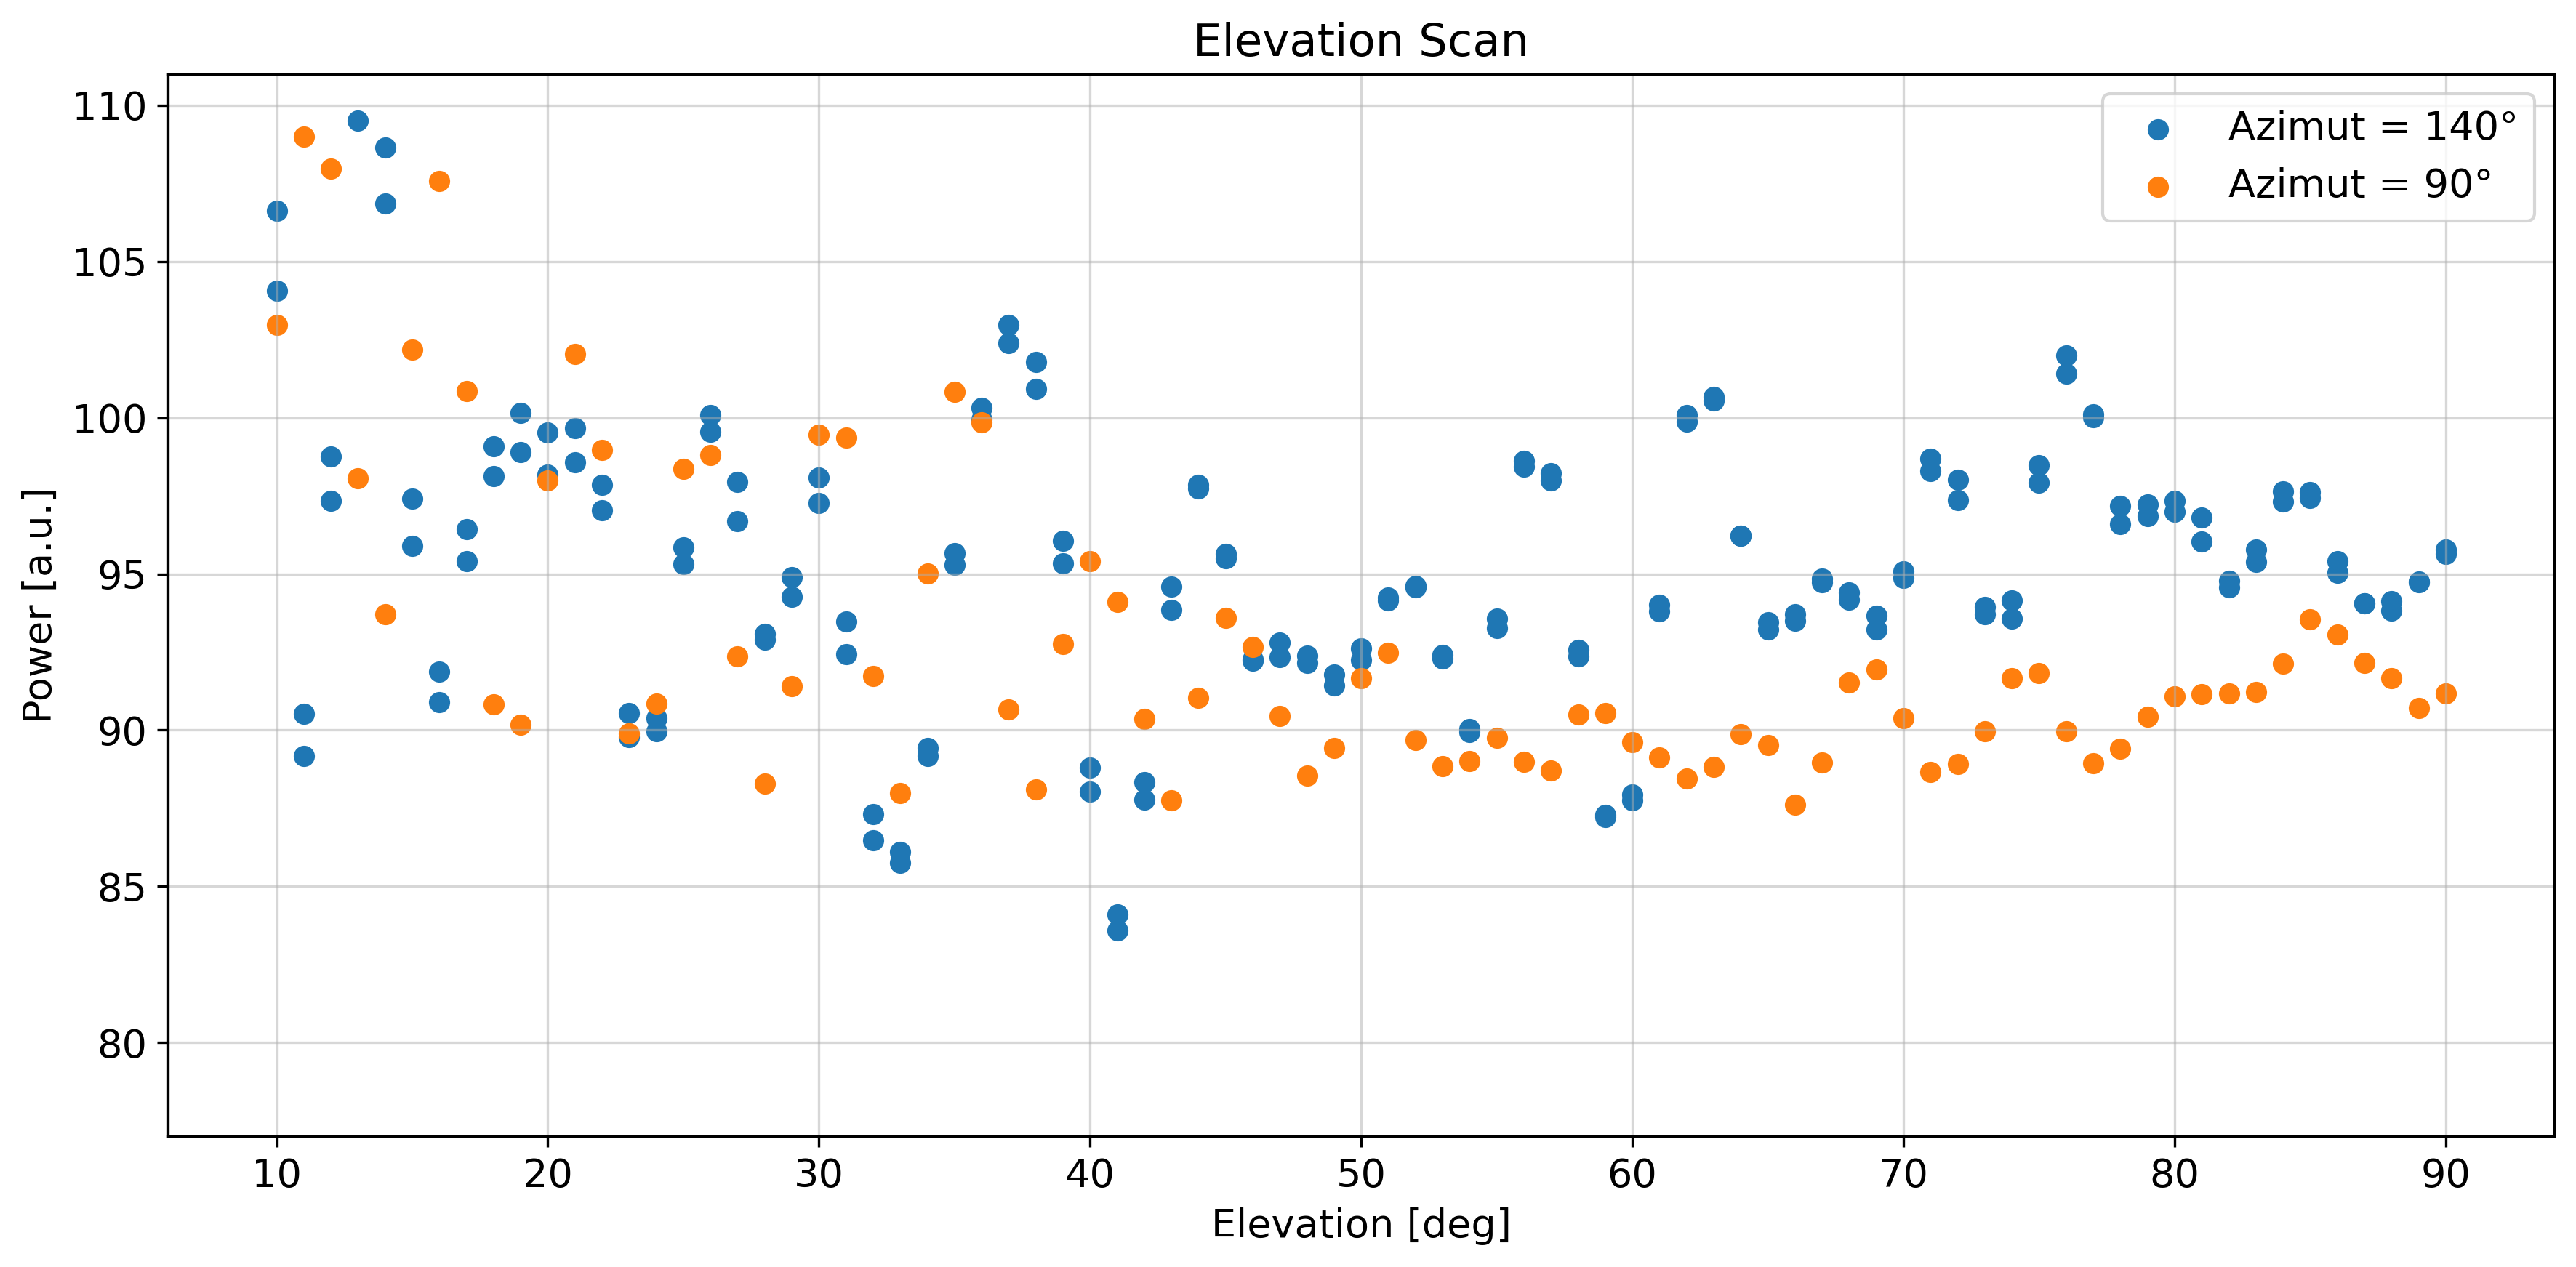
\includegraphics[width=\linewidth]{assets/elev_scan_day.png}
    \caption{Elevation Scan \texttt{02.10.2025 13:00 MESZ}}
\end{subfigure}
\caption{Elevation Scans at different times of the day}
\label{fig:elev_scan}
\end{figure}

%We notice that, both during the day and at night, the signal is stronger for low elevations. During the night we notice that additionally the signal gets stronger as we approach the zenith.

%To investigate this further we looked at the celestial bodies that where near the zenith during that time. A screenshot of this, taken in Stellarium is shown in figure \ref{fig:stellarium}. We notice, that the milky way is in the zenith during our time of measurement.
%
%\begin{figure}[H]
%    \centering
%    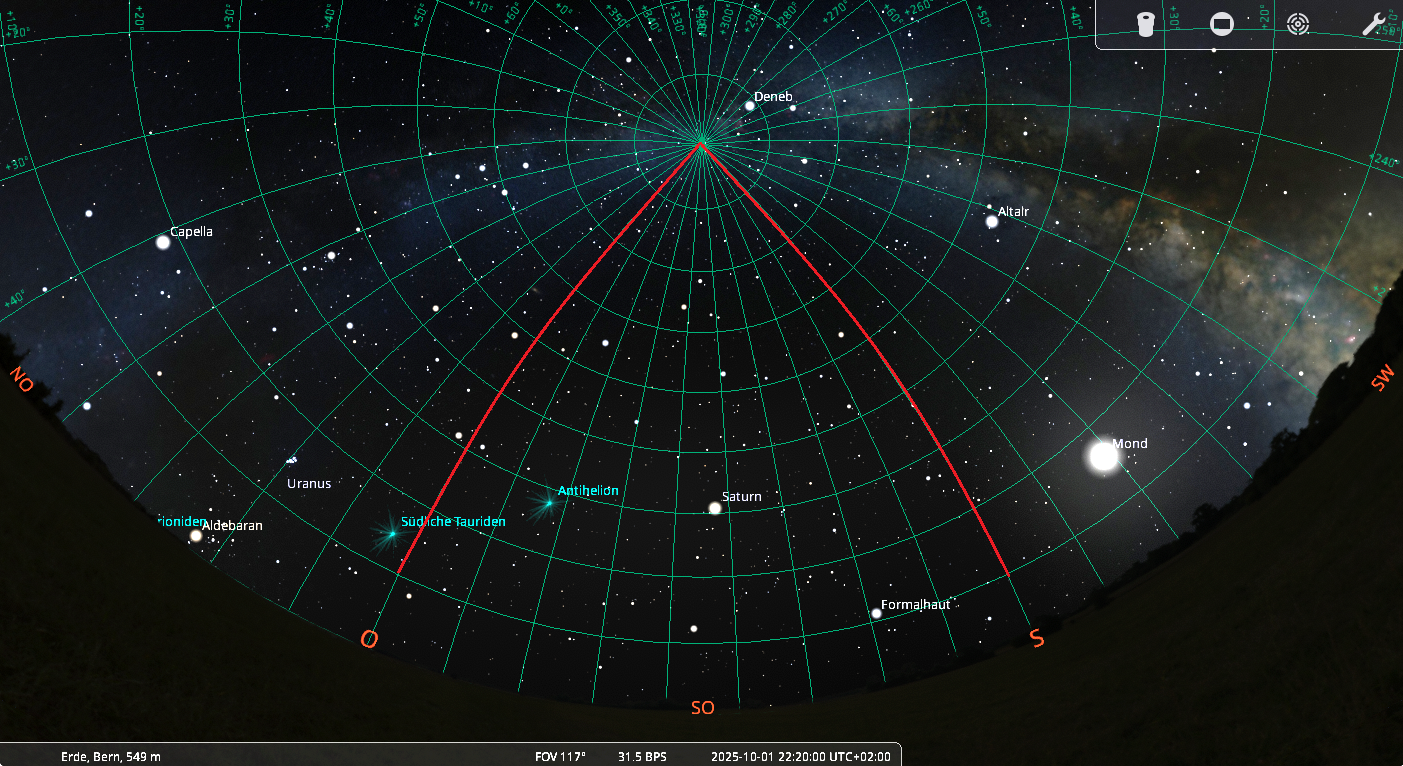
\includegraphics[width=0.6\linewidth]{assets/ElevationScan_Az90_Az180_251001_2220MESZ.png}
%    \caption{View of the sky at \texttt{01.10.2025 22:20 MESZ}}
%    \label{fig:stellarium}
%\end{figure}

%In figure \ref{fig:elev_spectra} we plot the Spectral power density both at day and night for an elevation where near the minima shown in figure \ref{fig:elev_scan}. We notice that during the day the spectra are a close match, and during the night we have a source with a frequency near the Carrier frequency, this would match with the \ce{H_I} we expect to be present in the milky-way.

%Because of this we think that the increase in Power that is only observed during the night is caused by the scan path intercepting the milky-way near the zenith.
%\begin{figure}[H]
%\centering
%\begin{subfigure}[t]{0.45\textwidth}
%    \centering
%    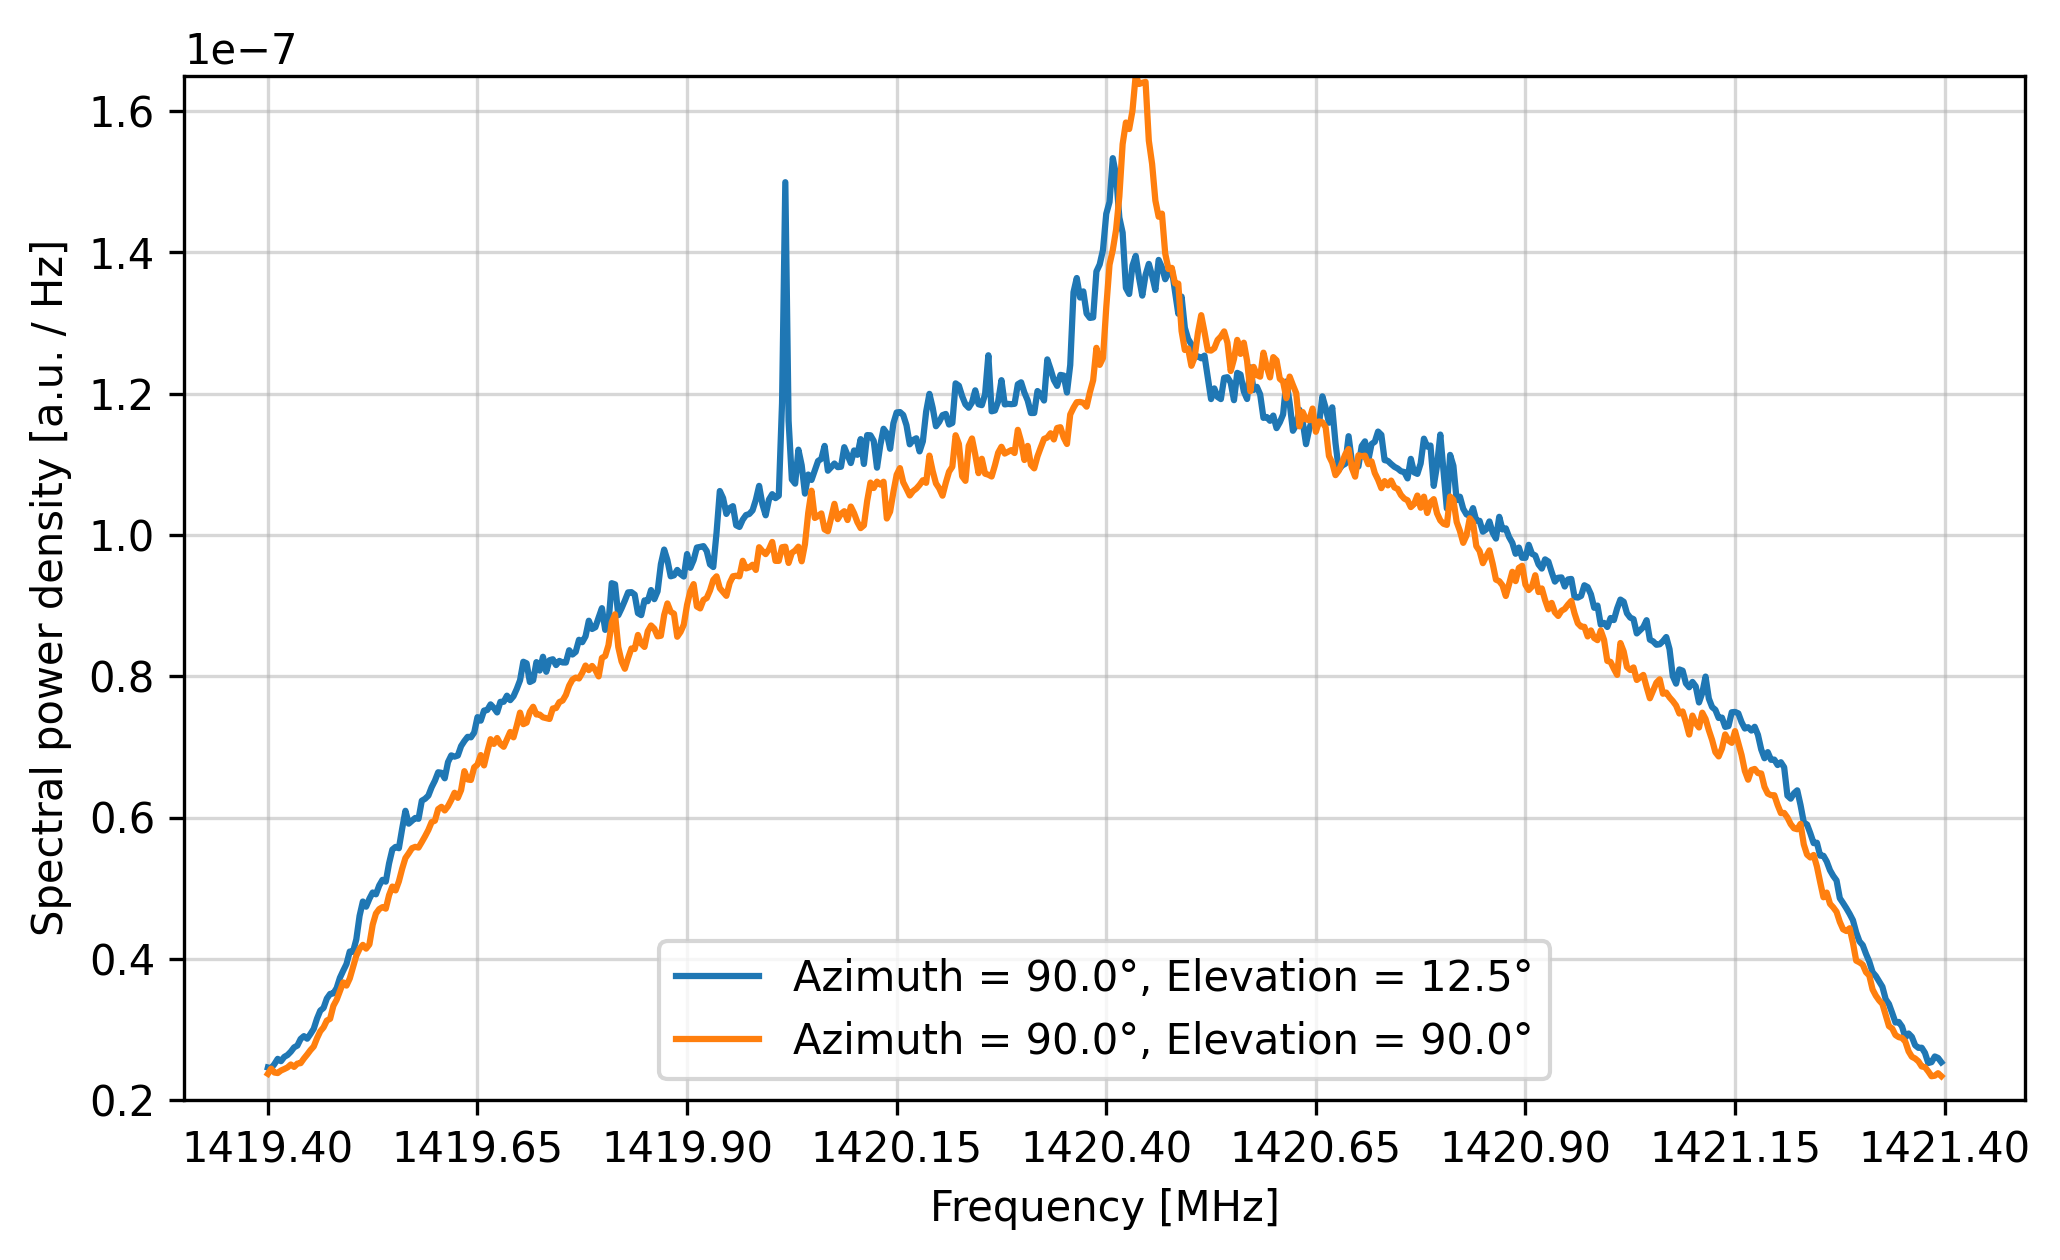
\includegraphics[width=\linewidth]{assets/elev_spectrum_night.png}
%    \caption{Spectra for two different elevations\\ \texttt{01.10.2025 22:35 MESZ}}
%\end{subfigure}
%\begin{subfigure}[t]{0.45\textwidth}
%    \centering
%    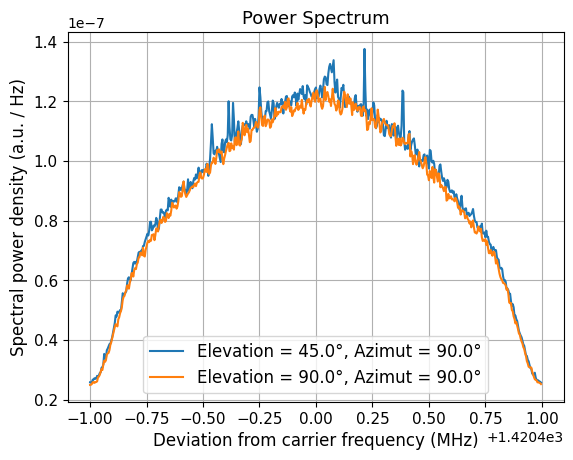
\includegraphics[width=\linewidth]{assets/elev_spectrum_day.png}
%    \caption{Spectra for two different elevations\\ \texttt{02.10.2025 13:00 MESZ}}
%\end{subfigure}
%\caption{Spectra at different Elevations and different times of the day}
%\label{fig:elev_spectra}
%\end{figure}
\subsection{Sun Scan}
We performed sun scans with two different settings.
A step size of \SI{0.5}{\degree} with a total scan width of \SI{20}{\degree} and a step size of \SI{0.1}{\degree} with a total scan width of \SI{10}{\degree}.
For each of the settings we performed a horizontal and a vertical scan centered around the sun.
The integrated power spectra are then each normalized by subtracting the minimum and then dividing with the (new) maximum.
These normalized values are shown in figures \ref{fig:sun_scan}

\begin{figure}[ht]
    \centering
    \begin{subfigure}[t]{0.45\linewidth}
        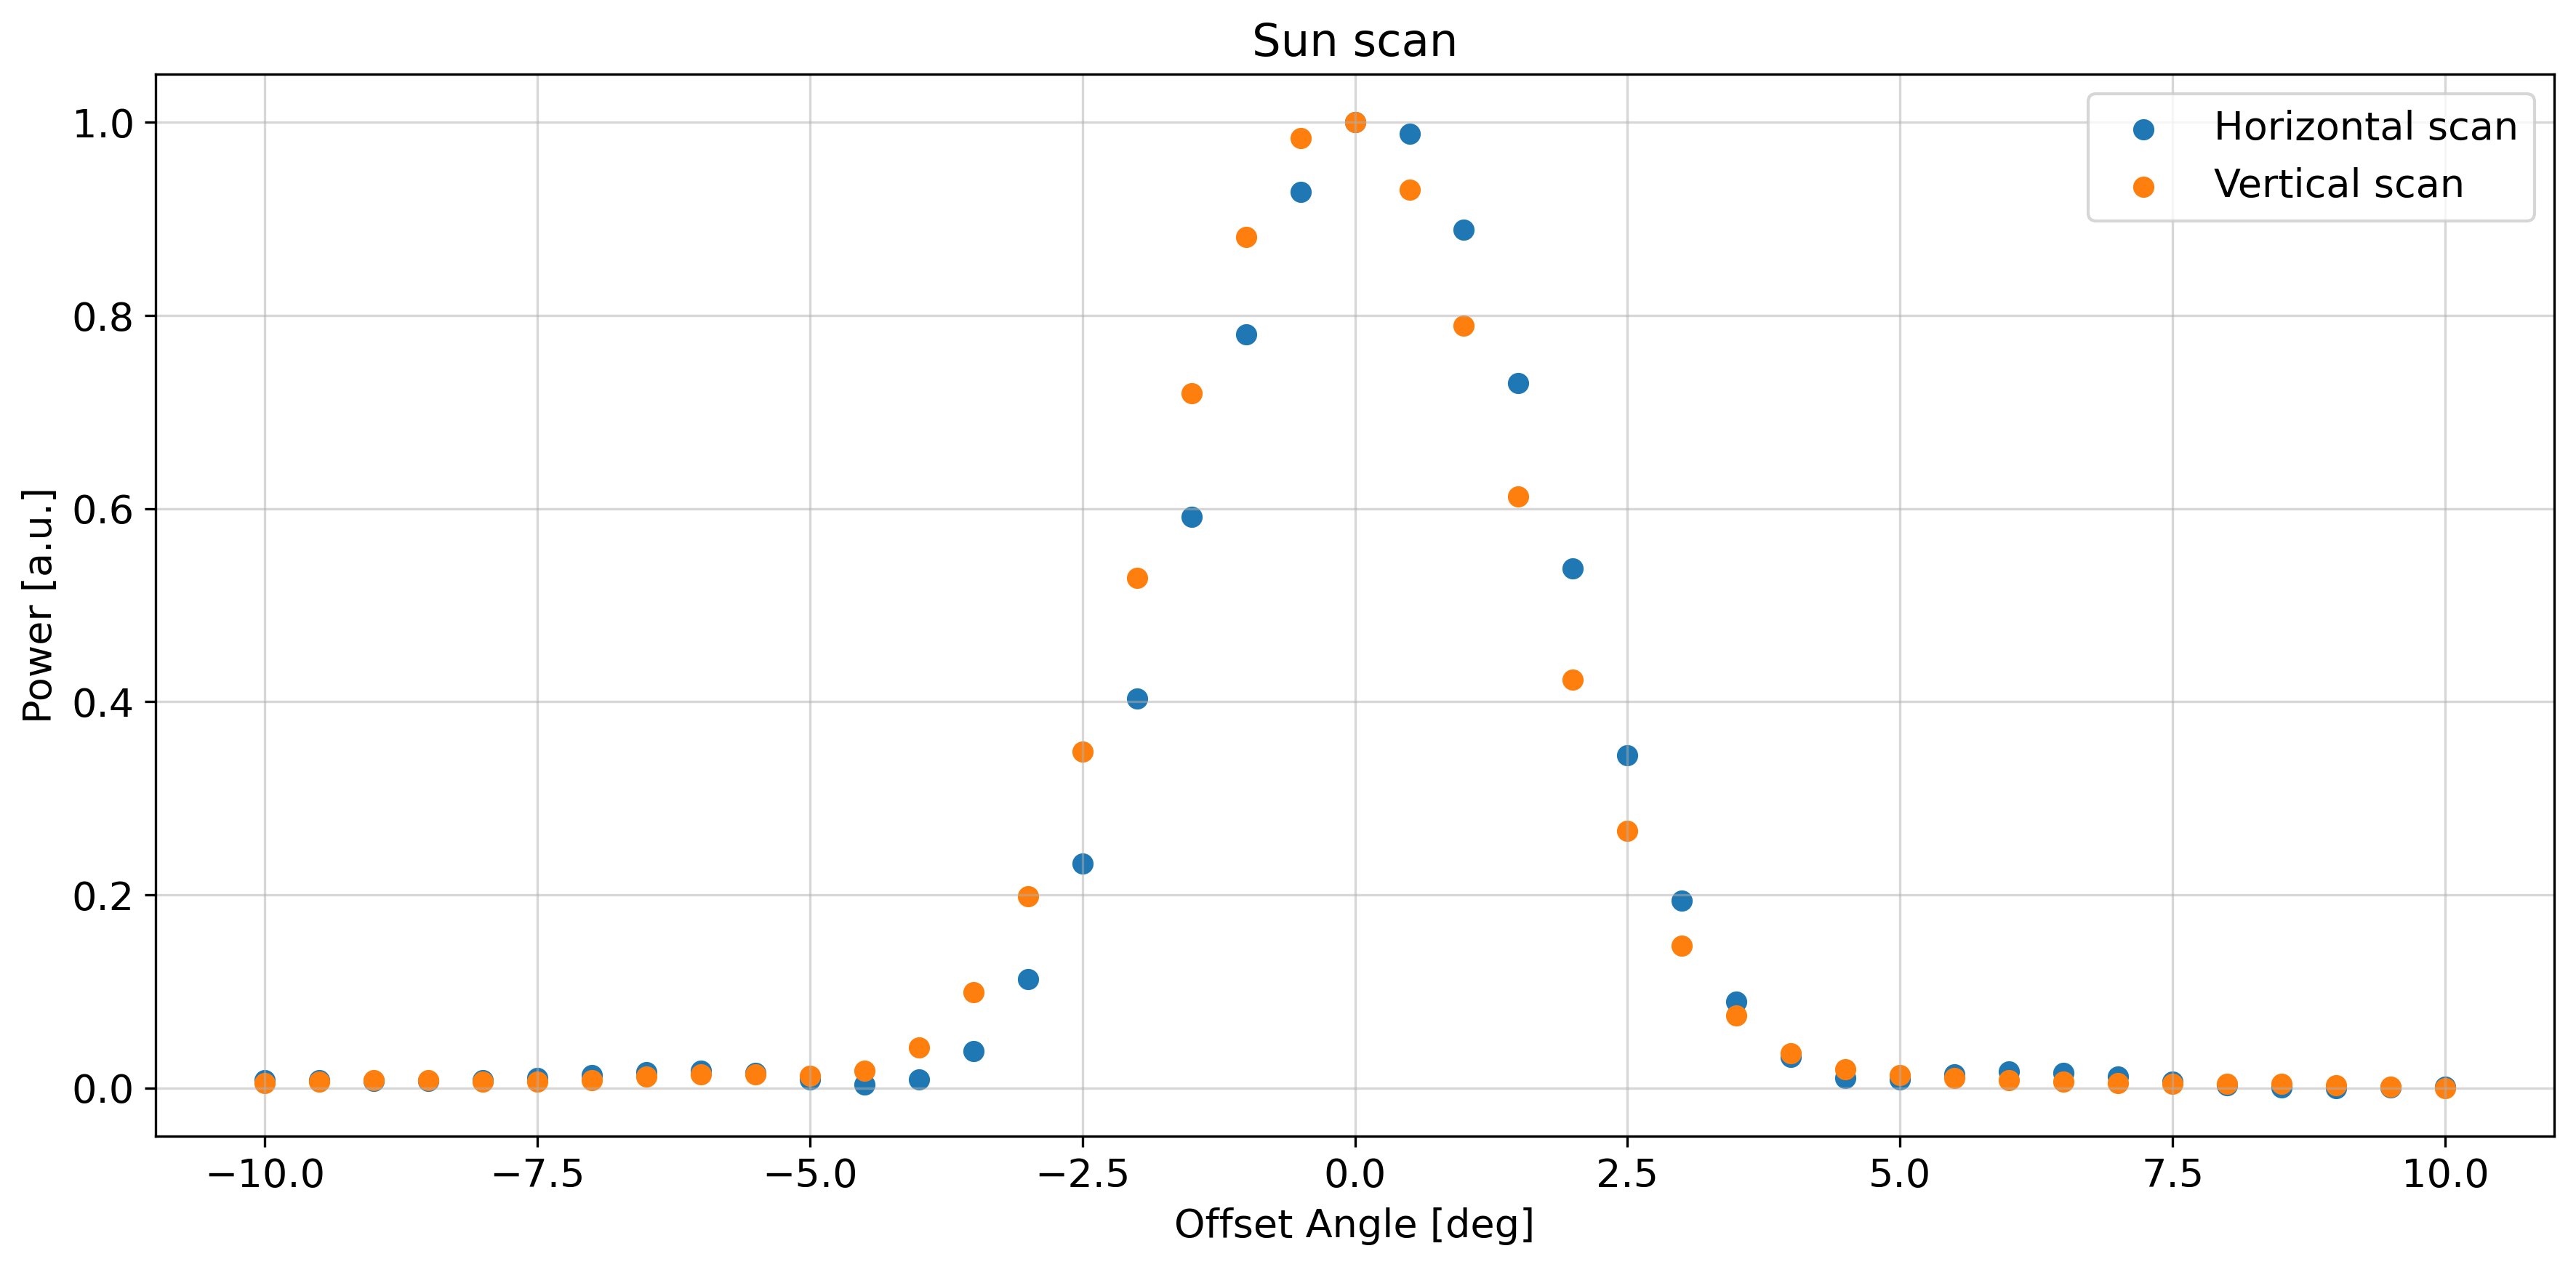
\includegraphics[width=\linewidth]{assets/sun_scan_low_res.png}
    \end{subfigure}
    \begin{subfigure}[t]{0.45\linewidth}
        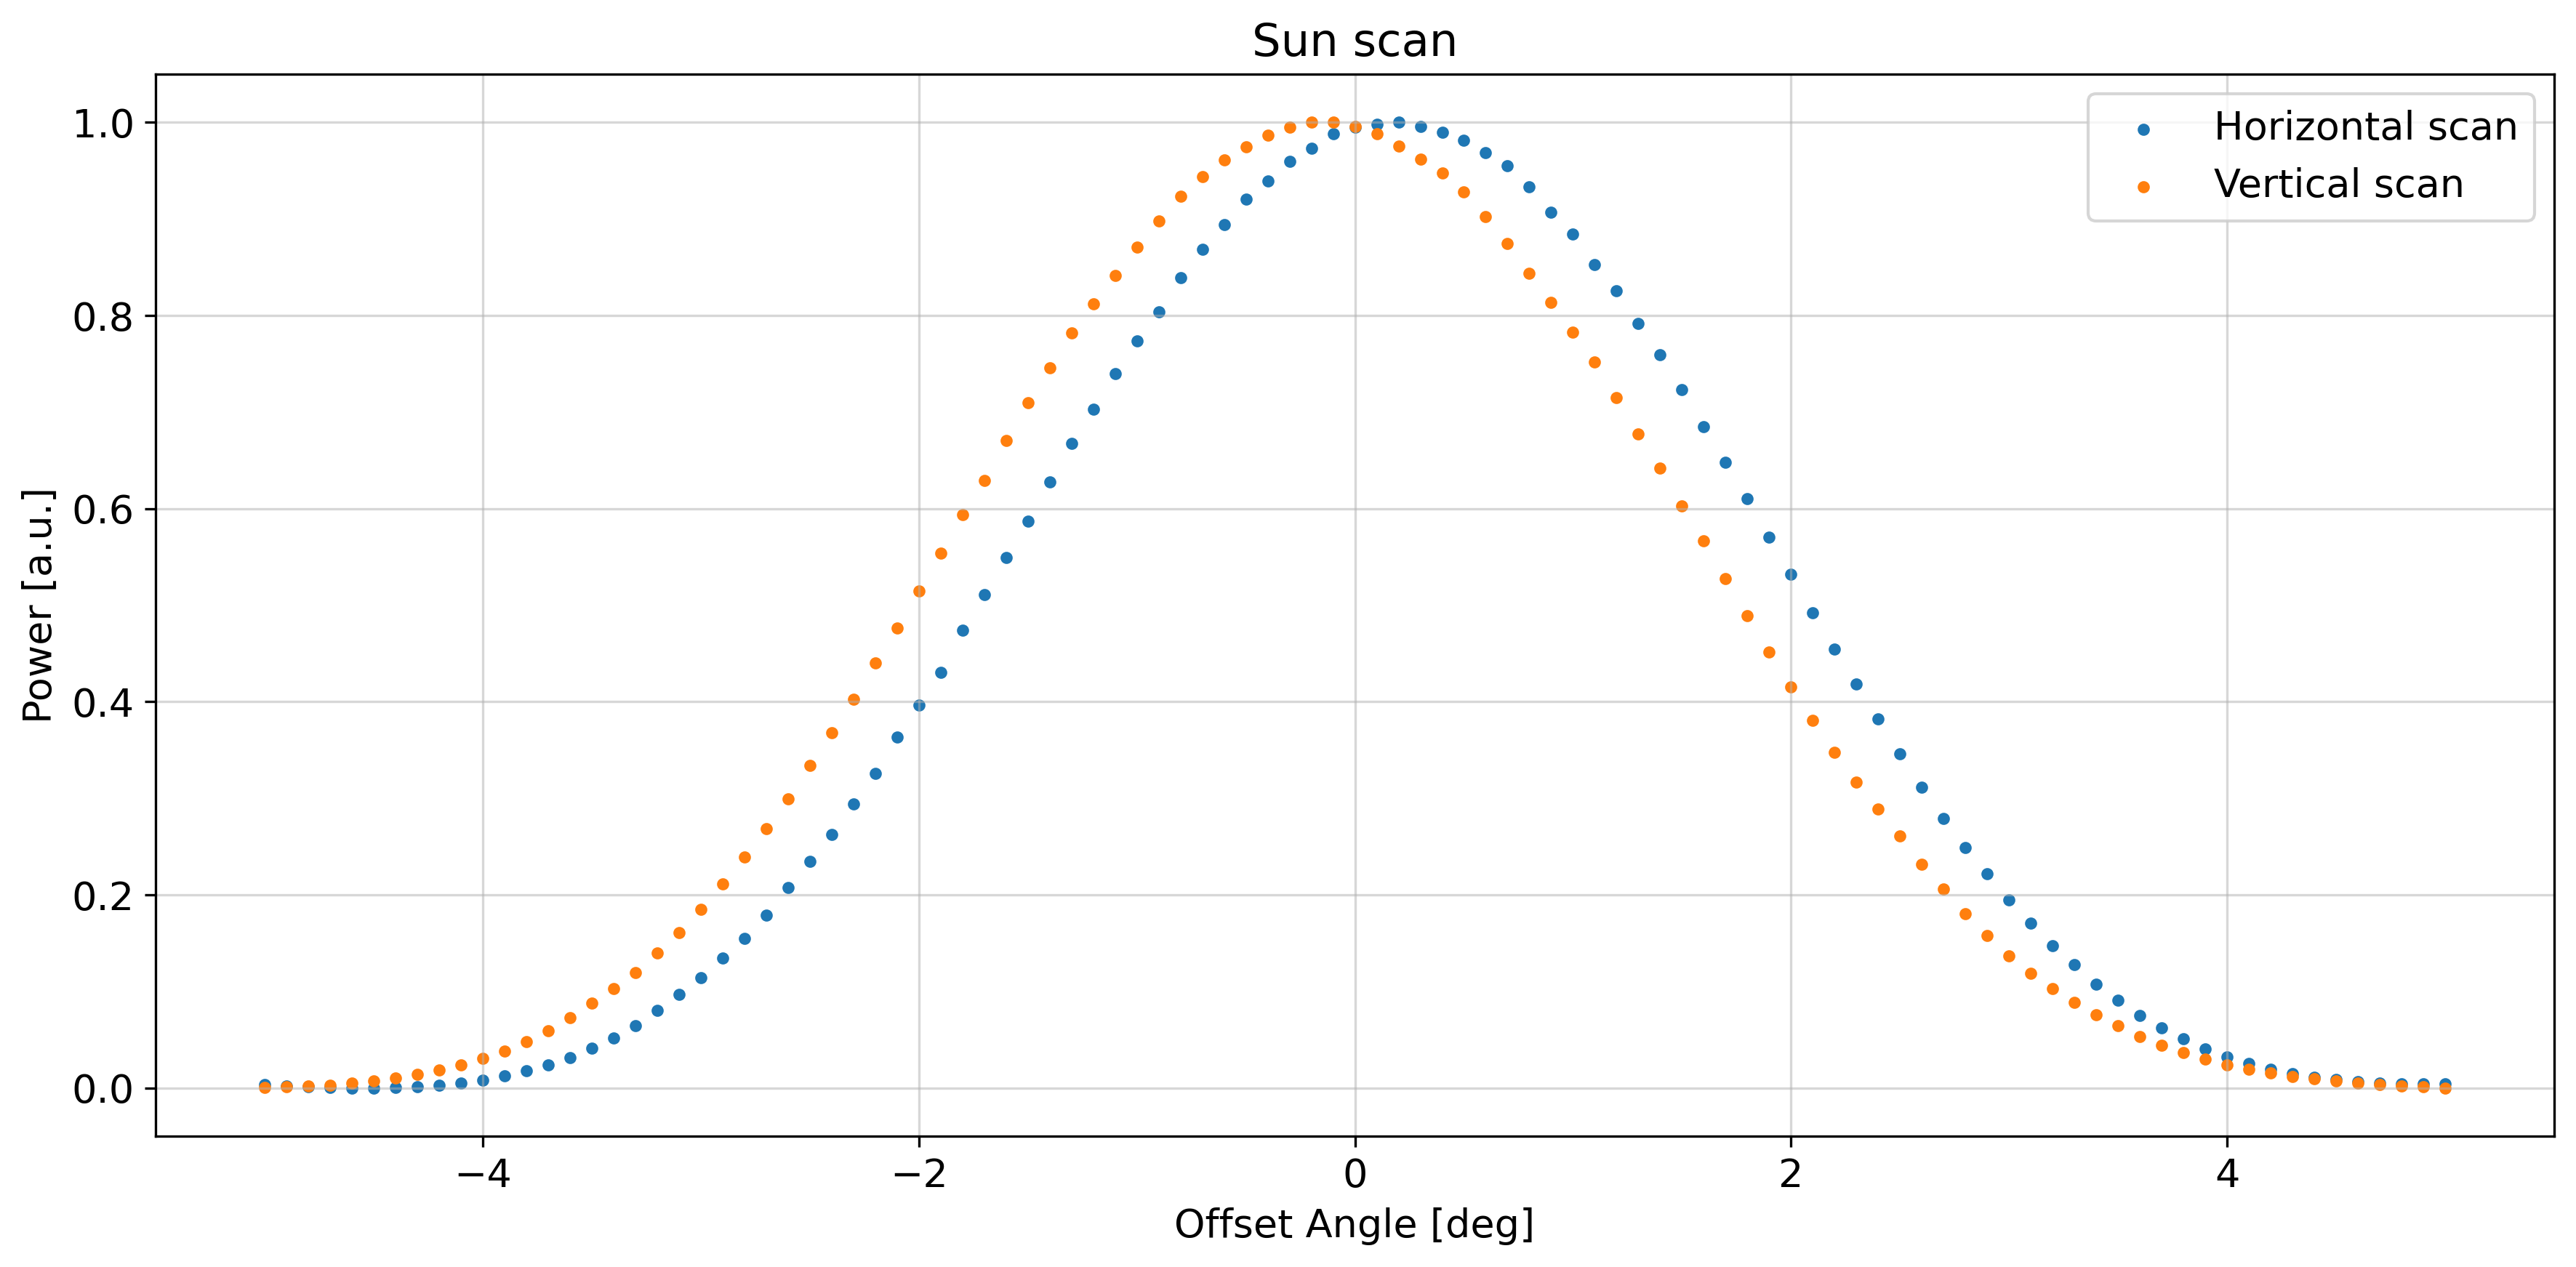
\includegraphics[width=\linewidth]{assets/sun_scan_high_res.png}
    \end{subfigure}
    \caption{Scan of the sun}
    \label{fig:sun_scan}
\end{figure}

The side bulbs are more visible when the normalizes power is shown logarithmically, this is shown in figure \ref{fig:sun_scan_log}
\begin{figure}[ht]
    \centering
    \begin{subfigure}[t]{0.45\linewidth}
        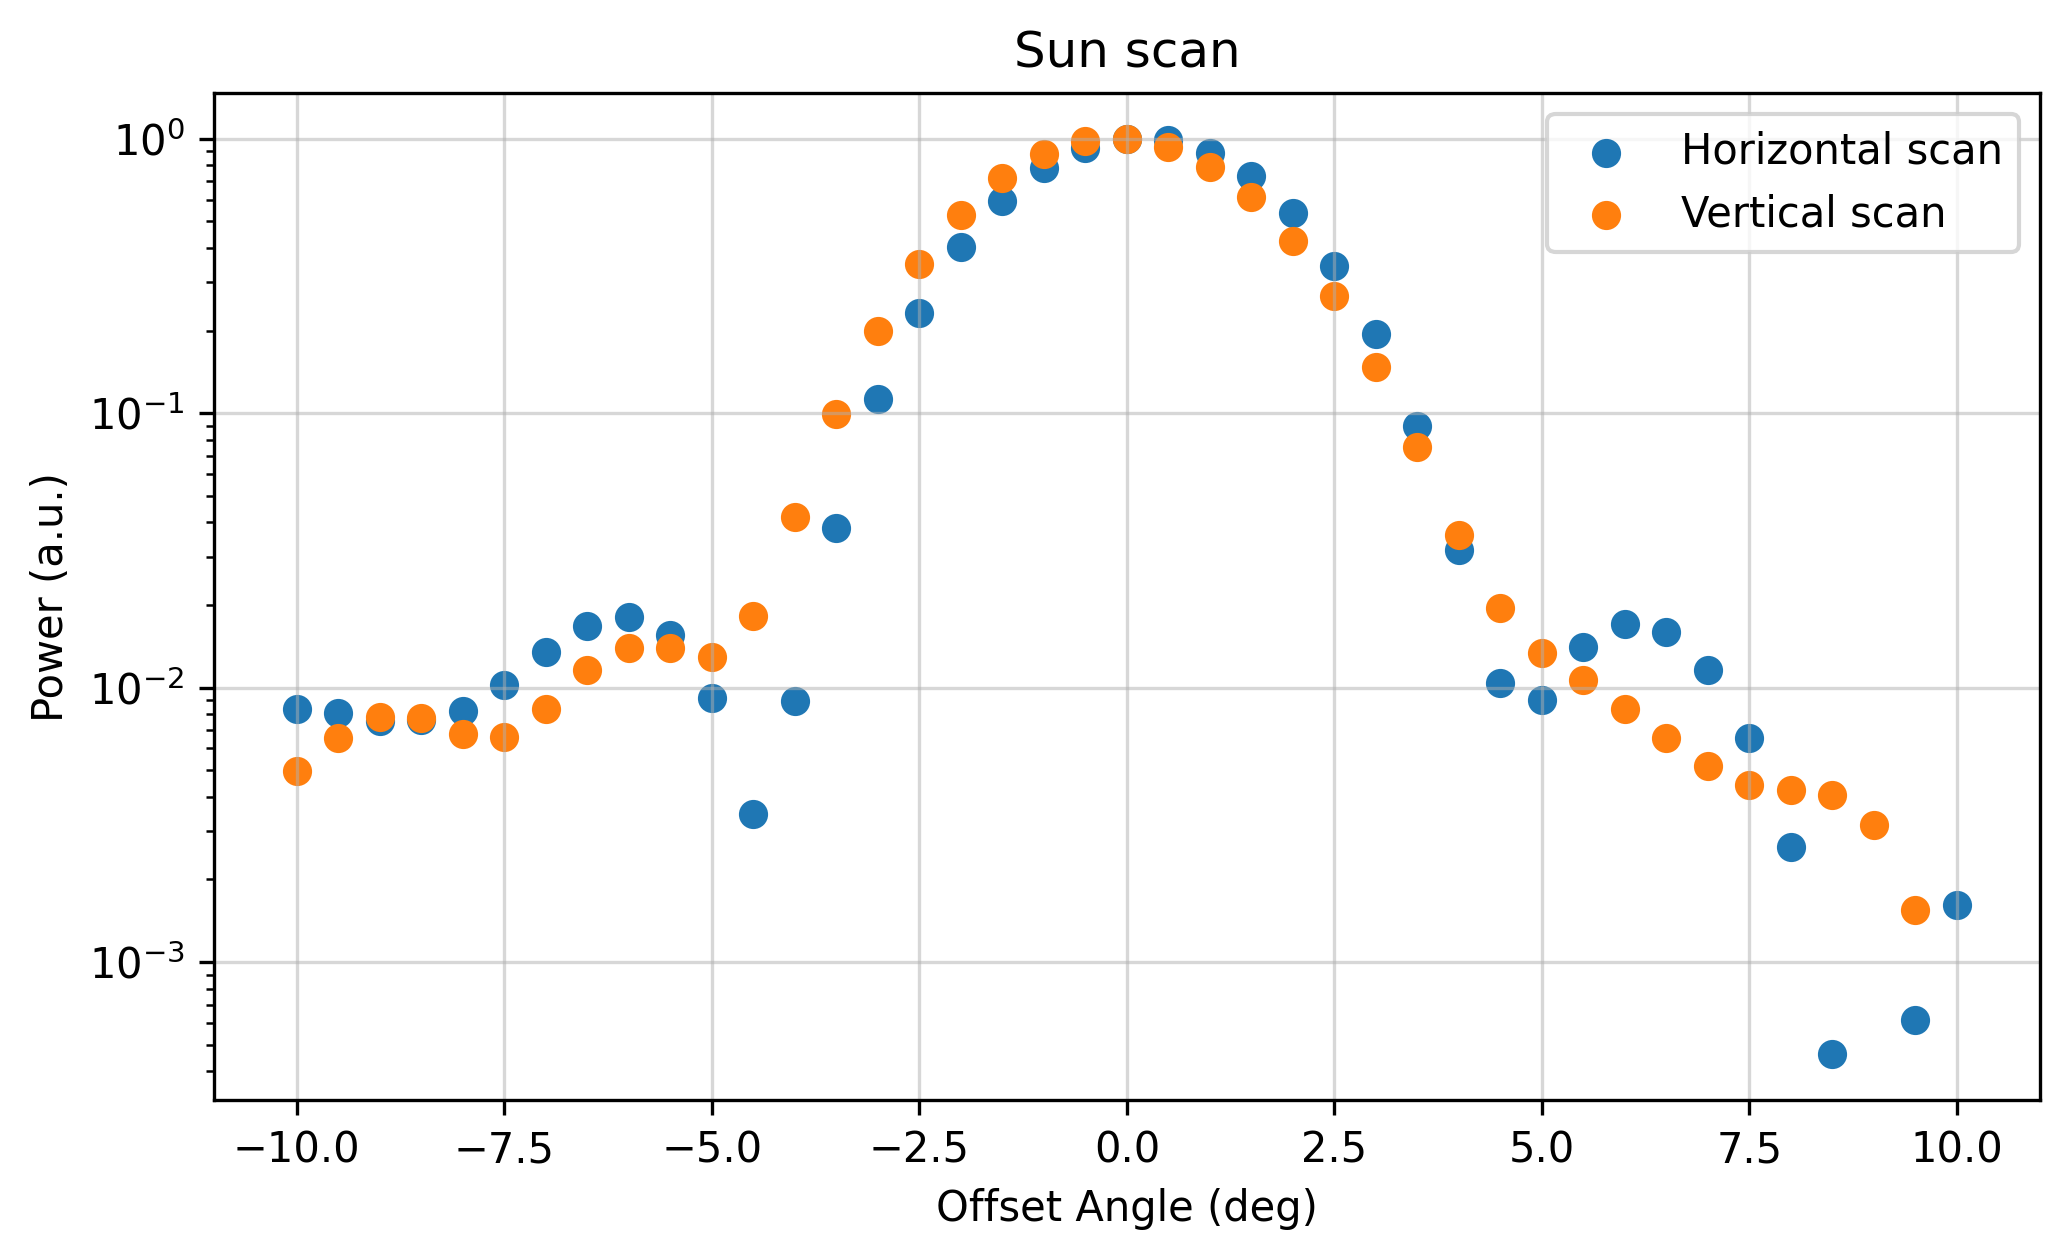
\includegraphics[width=\linewidth]{assets/sun_scan_low_res_log.png}
    \end{subfigure}
    \begin{subfigure}[t]{0.45\linewidth}
        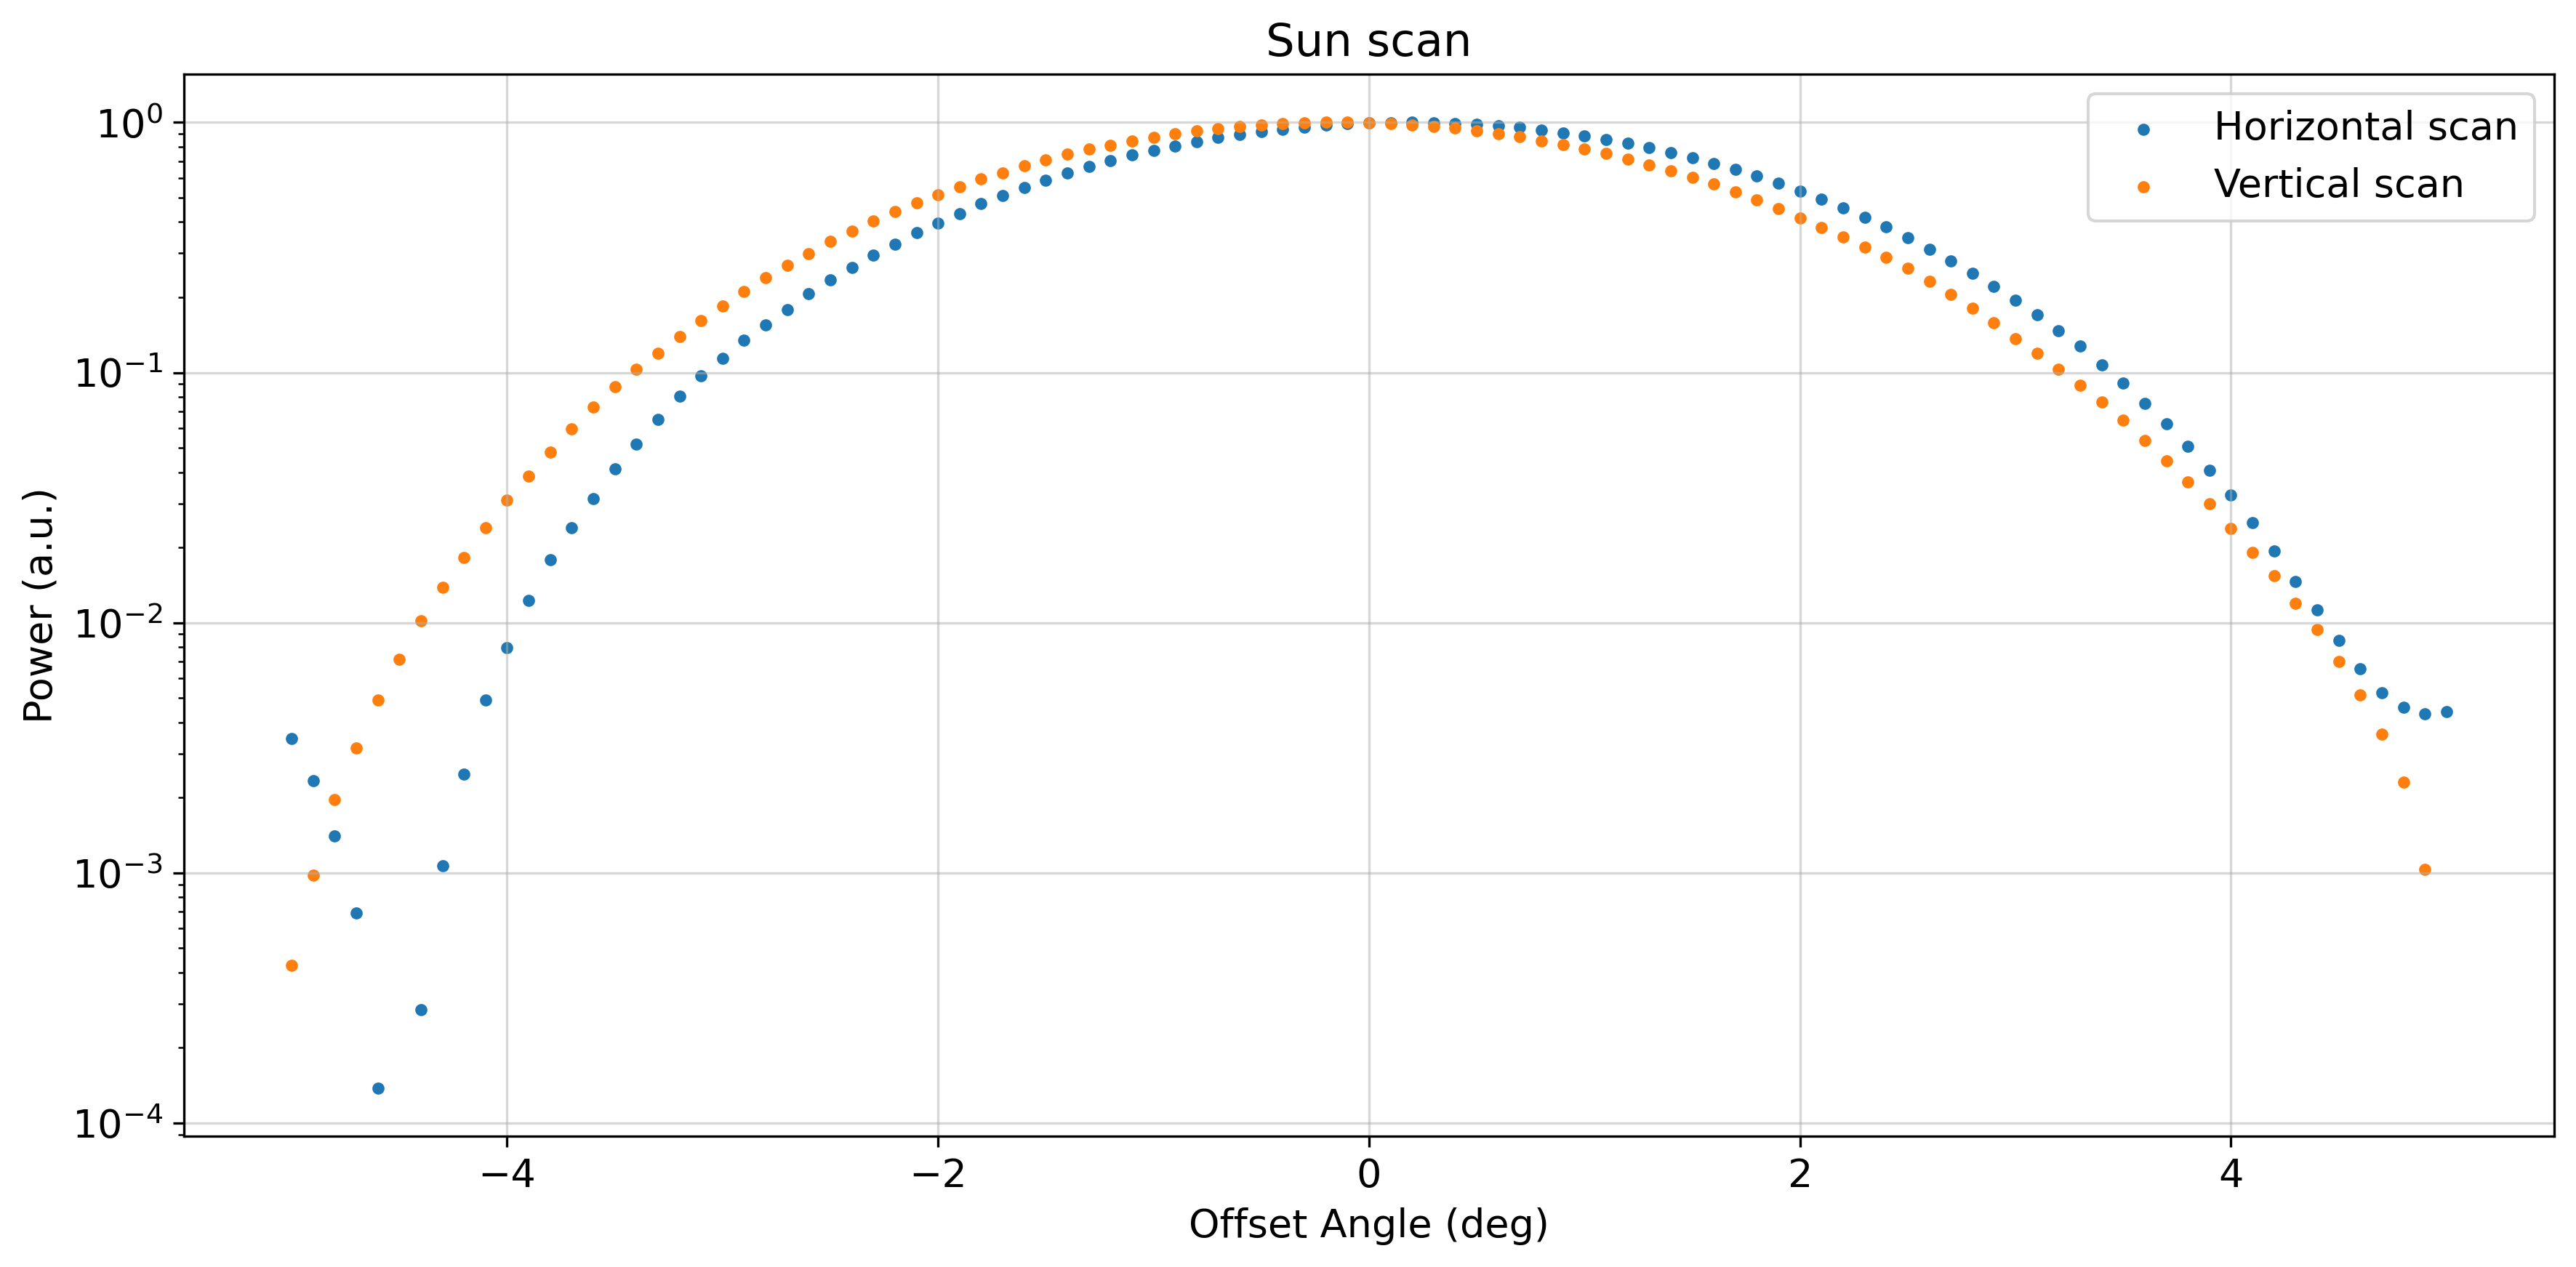
\includegraphics[width=\linewidth]{assets/sun_scan_high_res_log.png}
    \end{subfigure}
    \caption{Scan of the sun with logarithmic scale}
    \label{fig:sun_scan_log}
\end{figure}

To determine the full width at half maximum (FWHM) we use the high resolution data and fit it to a gaussian.
The equation describing the functional model is
\begin{equation}
    P = \exp{\left(-\frac{(\theta-\theta_0)^2}{2\sigma^2}\right)}
\end{equation}.
The model can then be fitted using iterative least squares as described in TODO: find good source. The FWHM can then be computed using \eqref{eq:FWHM}. 
The resulting values are shown in table \ref{tab:params} and figure \ref{fig:sun_scan_fit}.
\begin{table}[ht]
    \centering
    \begin{tabular}{lrrr}
        \toprule
        Direction & FWHM & $ \sigma $ & $ \theta_0 $\\
        \midrule
        Horizontal & \SI{3.720(0.010)}{\degree} & \SI{1.581(0.005)}{\degree} & \SI{0.179(0.006)}{\degree} \\
        Vertical & \SI{3.751(0.009)}{\degree} & \SI{1.593(0.004)}{\degree} & \SI{-0.131(0.005)}{\degree} \\
        \bottomrule
    \end{tabular}
    \caption{functional model parameters from least squares fit}
    \label{tab:params}
\end{table}
\begin{figure}[ht]
    \centering
    \begin{subfigure}[b]{0.45\textwidth}
        \centering
        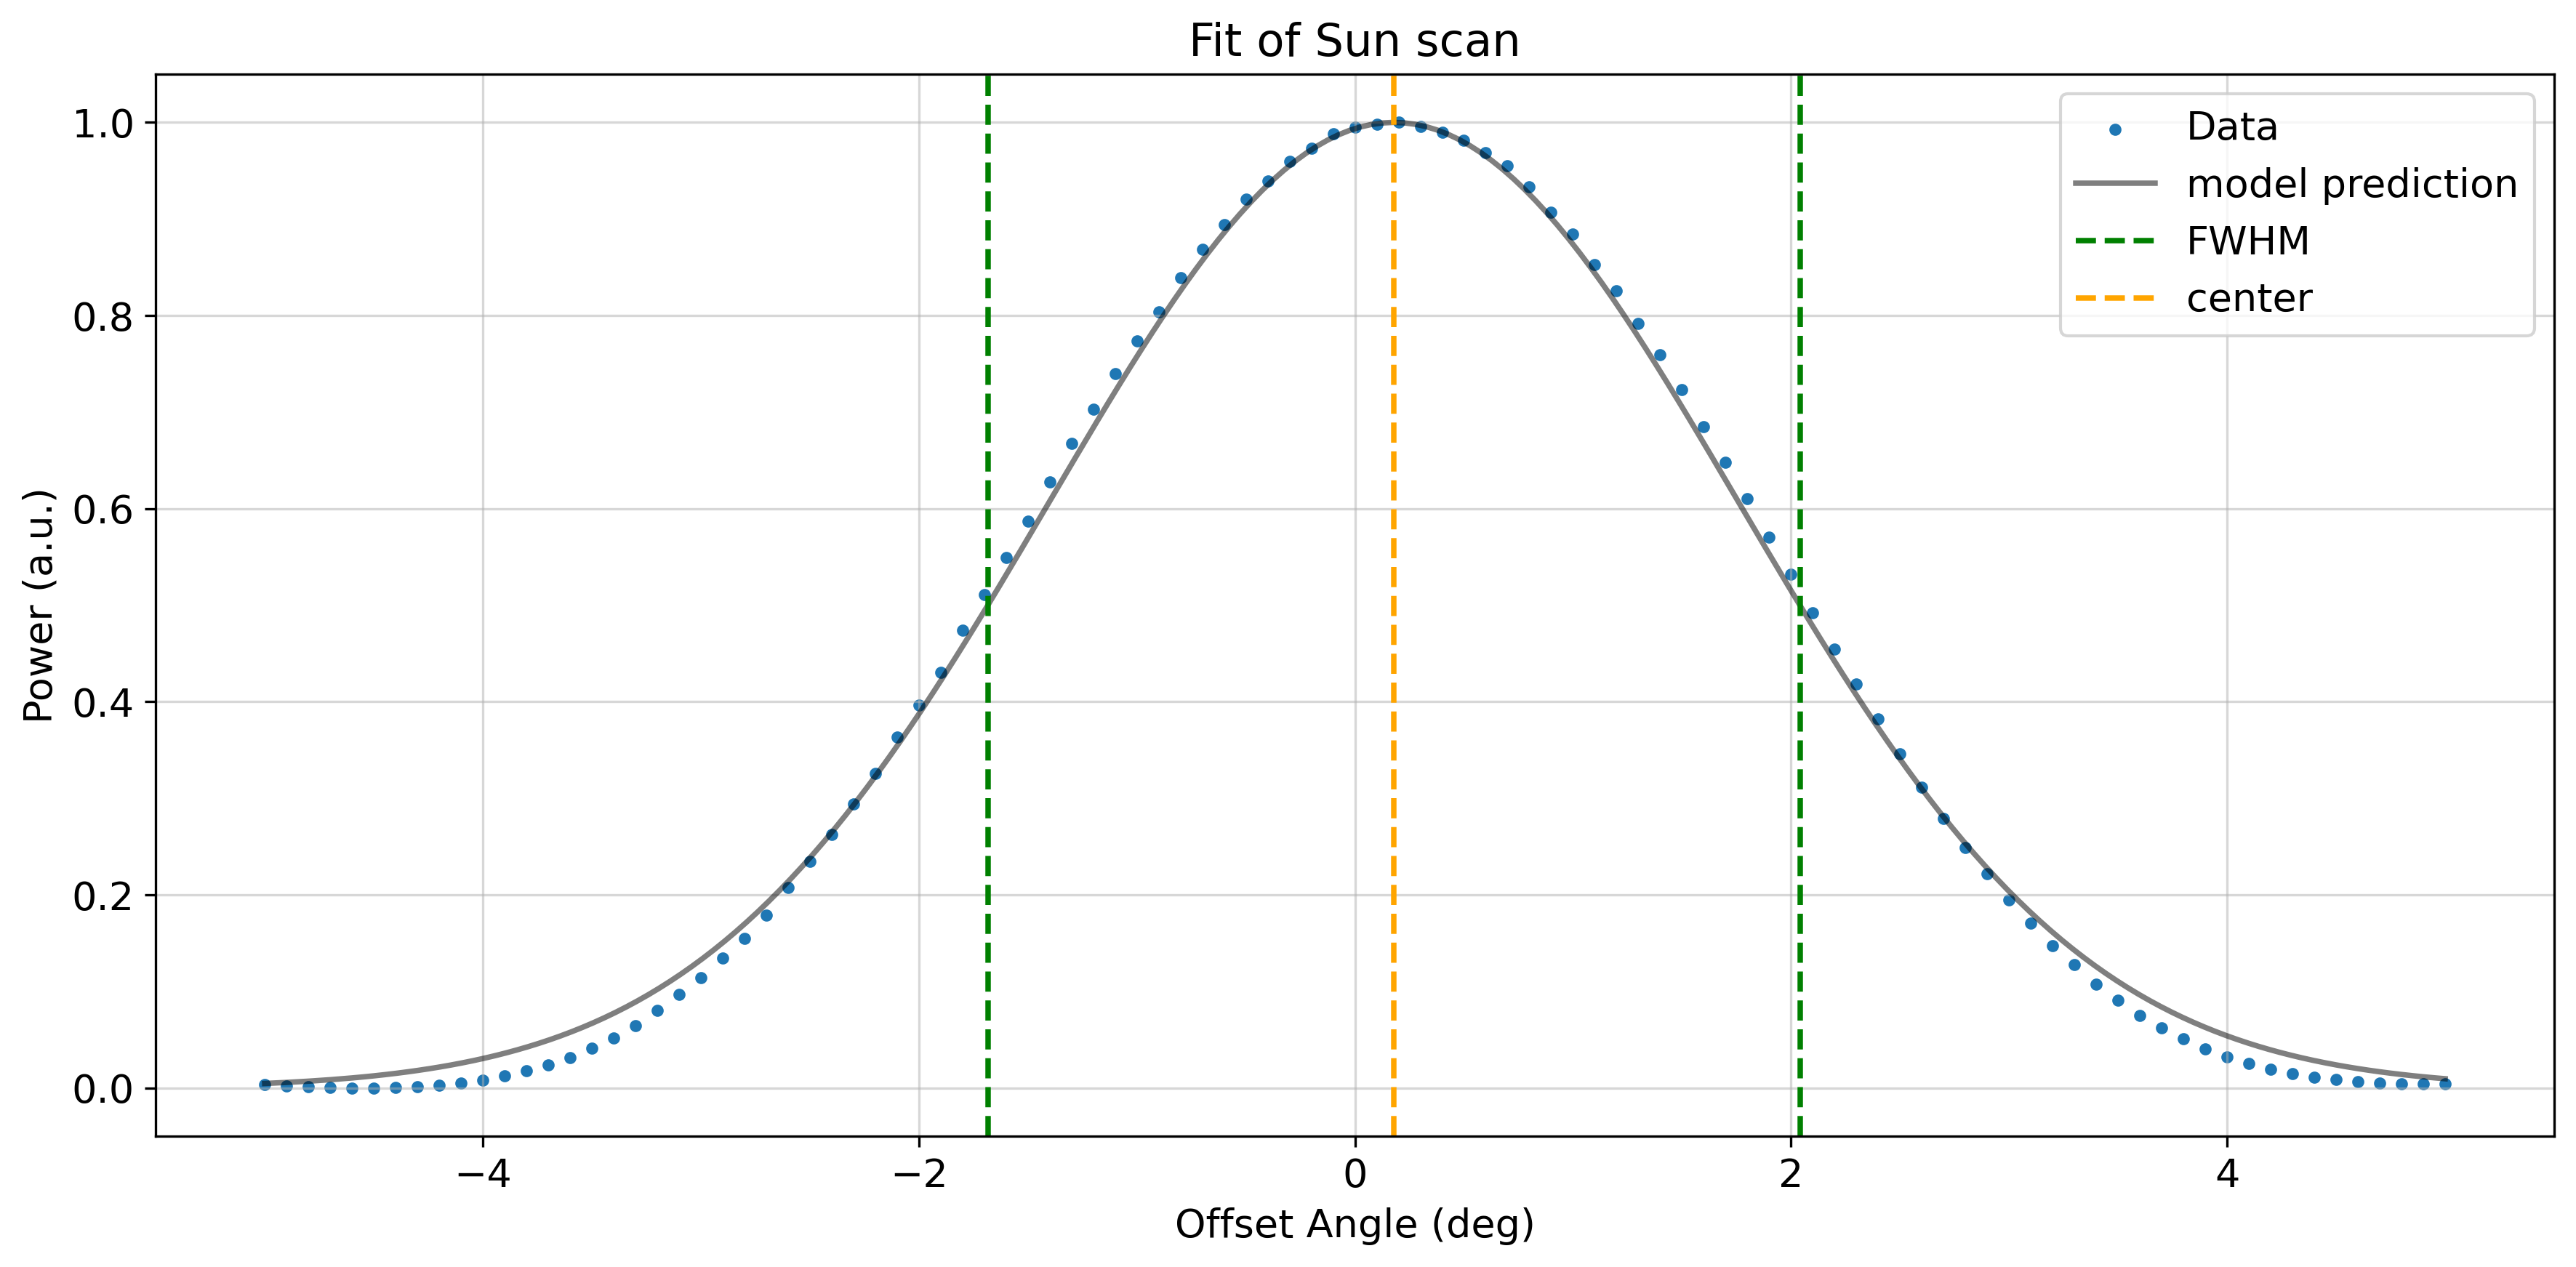
\includegraphics[width=\textwidth]{assets/sun_scan_fit_h.png}
        \caption{Horizontal fit to the data}
        \label{fig:sun_fit_h}
    \end{subfigure}
    \hfill
    \begin{subfigure}[b]{0.45\textwidth}
        \centering
        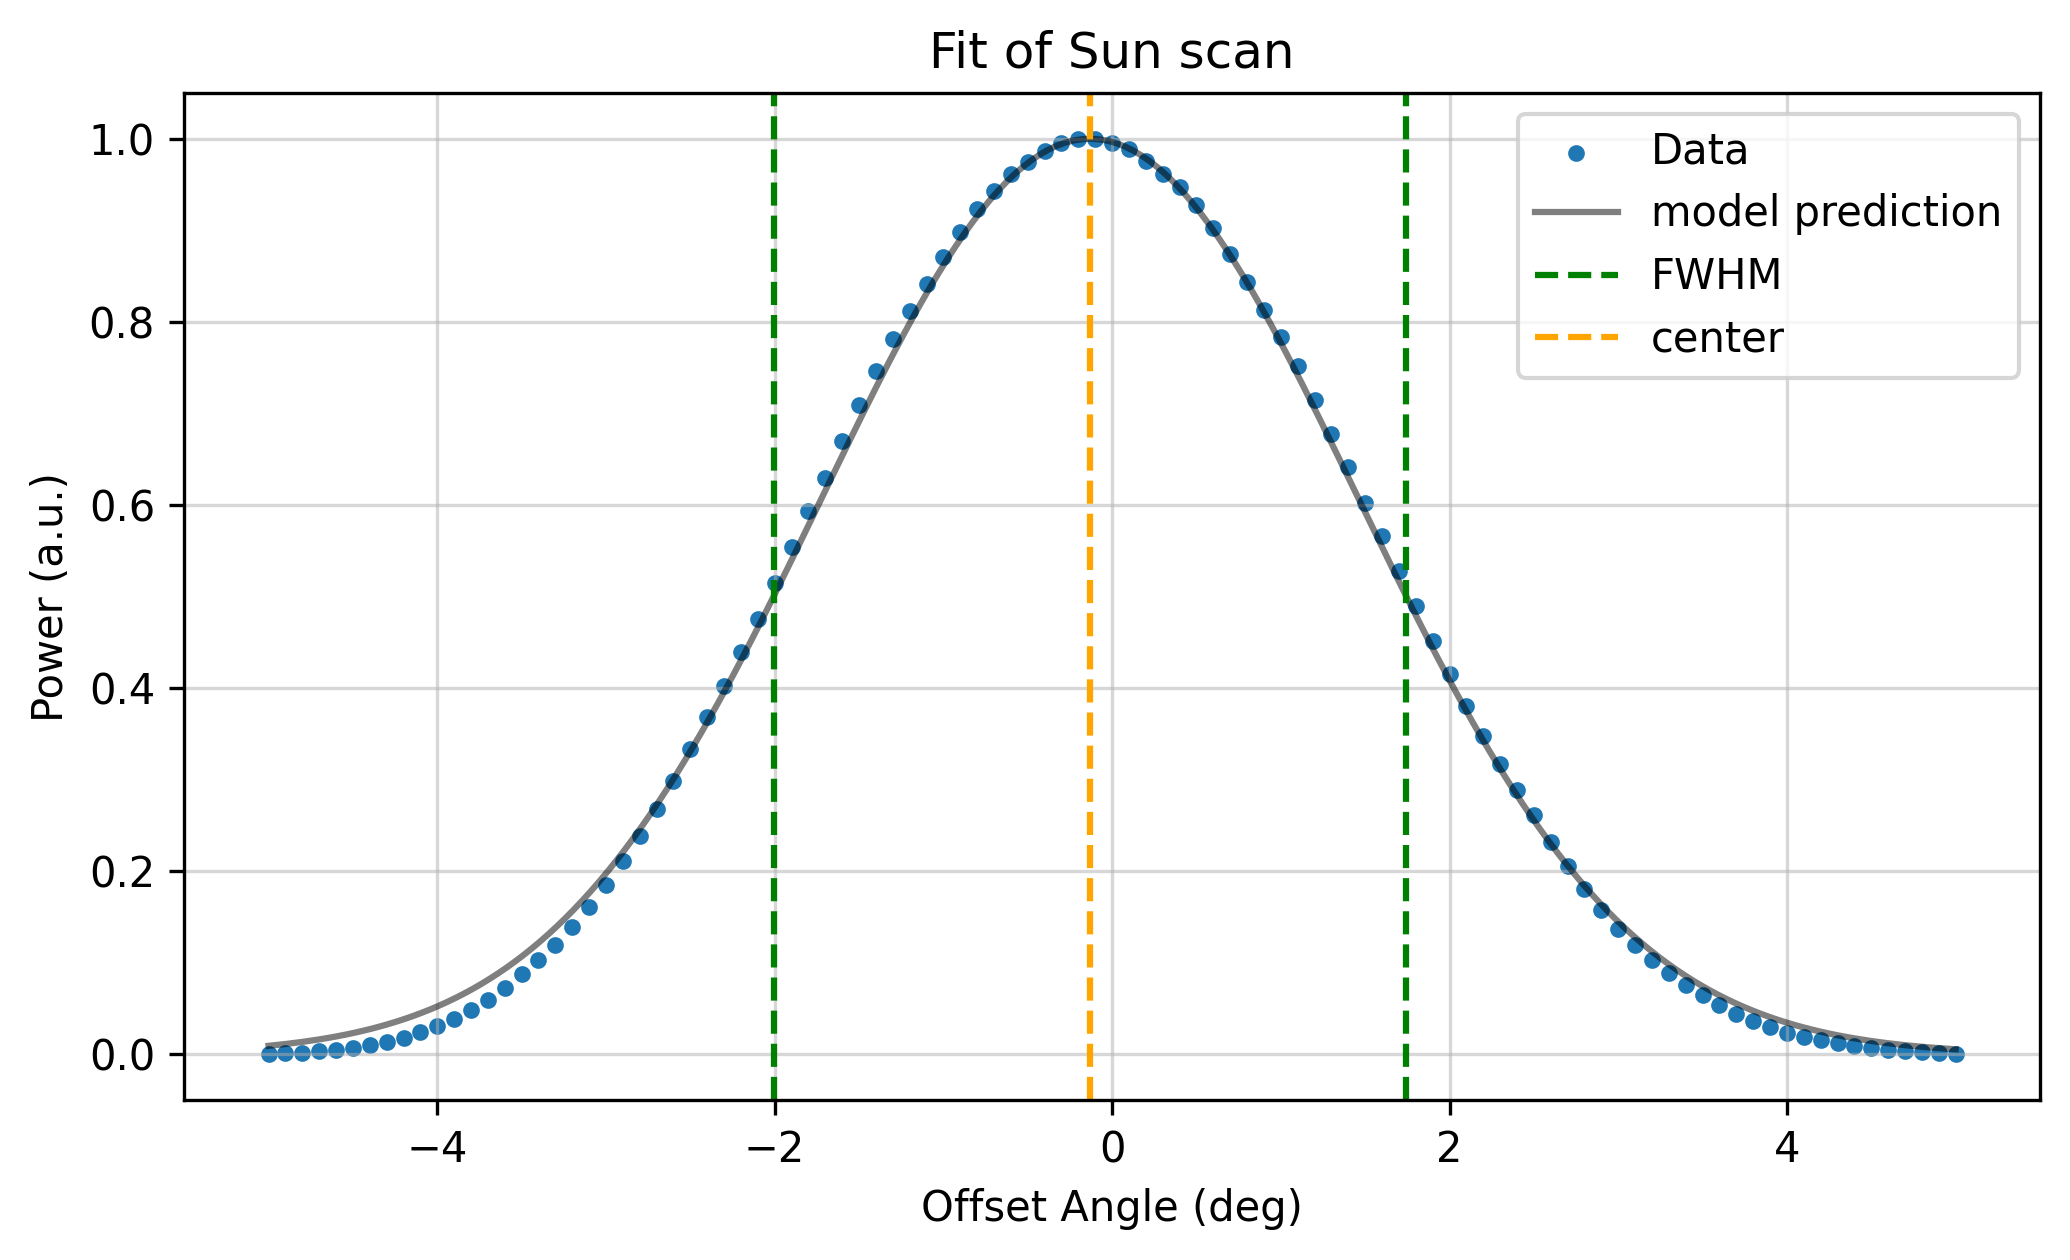
\includegraphics[width=\textwidth]{assets/sun_scan_fit_v.png}
        \caption{Vertical}
        \label{fig:sun_fit_v}
    \end{subfigure}
    \caption{;alkdsf}
    \label{fig:sun_scan_fit}
\end{figure}
If we compare the values for the FWHM from table \ref{tab:params} with those from table \ref{tab:ang_res}
we find that the theoretical values do not lie withing the error bounds of the measured value.
We think the reason for this discrepancy is a combination of
\begin{itemize}
    \item Unknown errors in the given constants $d = \SI{4}{m}$ and $\eta = 0.5$, especially $\eta$ since it is not trivial to measure.
    \item Invalid assumption that the main bulb is gaussian.
    \item Invalid assumption that the solid angle that is not in the main bulb is negligible.
    \item Invalid assumption that the contribution from the integral in \eqref{eq:gauss_integral} of the gaussian with $\theta > \pi$ is negligible.
\end{itemize}
\subsection{Calibration and Sun Temperature}
\subsection{Milky Way Scan}

\subsubsection{Observation time}
From our observation spot in Bern, we had to plan the observation time to get the best possible overview of the Milky Way with a wide range in the galactic longitude. In October, when we did this measurments, the maximum elevation of the galactic center is around 13° (in south) at 18:30 MESZ. However, limitations in the field of view of the SRT had to be considered to choose the best observation time:

\begin{itemize}
    \item At 18:30 MESZ, the galactic center ($l_g=\SI{0}{\degree}$) could be included in the scan but at galactic longitudes of $l_g>\SI{120}{\degree}$, the SRT run in the lower azimuth limit from EXWI building at around 40° (north east).
    \item At later times, the galactic center is already descending and but the higher galactic longitudes are moving inside visible area of the SRT.
    \item At 22:00 MESZ, the galactic center is at the horizon and no more visible but the galactic plane is almost perpendicular to the horizontal plane and it is in the visible area of the SRT up to galactic longitude $l_g=\SI{180}{\degree}$. Only limitation is the main building of the University Bern, that covers the view partially. We decided to do the scan at this time. 
\end{itemize}
    
The scan path is illustrated in figure \ref{fig:mw_scan_stellarium}. We chose the scan path start at galactic longitude of 10° and end at 170° to avoid lower elevations than 10° as the noise level of the ground thermal radiation is dominating there.


\begin{figure}[H]
    \centering
    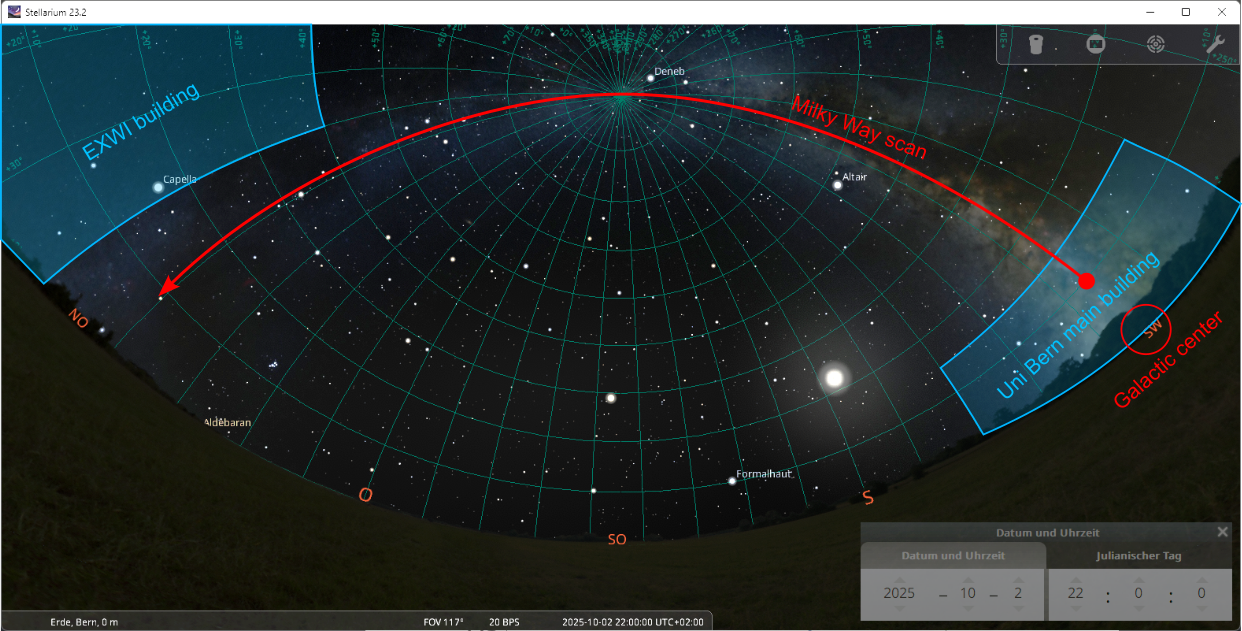
\includegraphics[width=12cm]{assets/stellariumView_edit.png}
    \caption{View of the Milky Way scan in Stellarium [XXX] with SRT field of view limitations (blue).}
    \label{fig:mw_scan_stellarium}
\end{figure}

\subsubsection{Measurement}
It was hard to find out, how to correctly set up the Lab View tool for a Milky Way scan, as the angular range input fields belong to azimuthal coordinates rather than galactic. Finally we found, that the tool uses wrong (mirrored) galactic coordinates (correct longitude is $l_g=\SI{360}{\degree}-l_{srt}$ to enter in the azimuth fields. We chose a step size of $\Delta l_g=\SI{0.25}{\degree}$ with 1000 ms integration time what resulted in a measurement time of 28 min to scan from 10° to 170° in galactic coordinates. Figure \ref{fig:mw_scan_polar} shows the scan path in a polar diagram:

\begin{figure}[H]
    \centering
    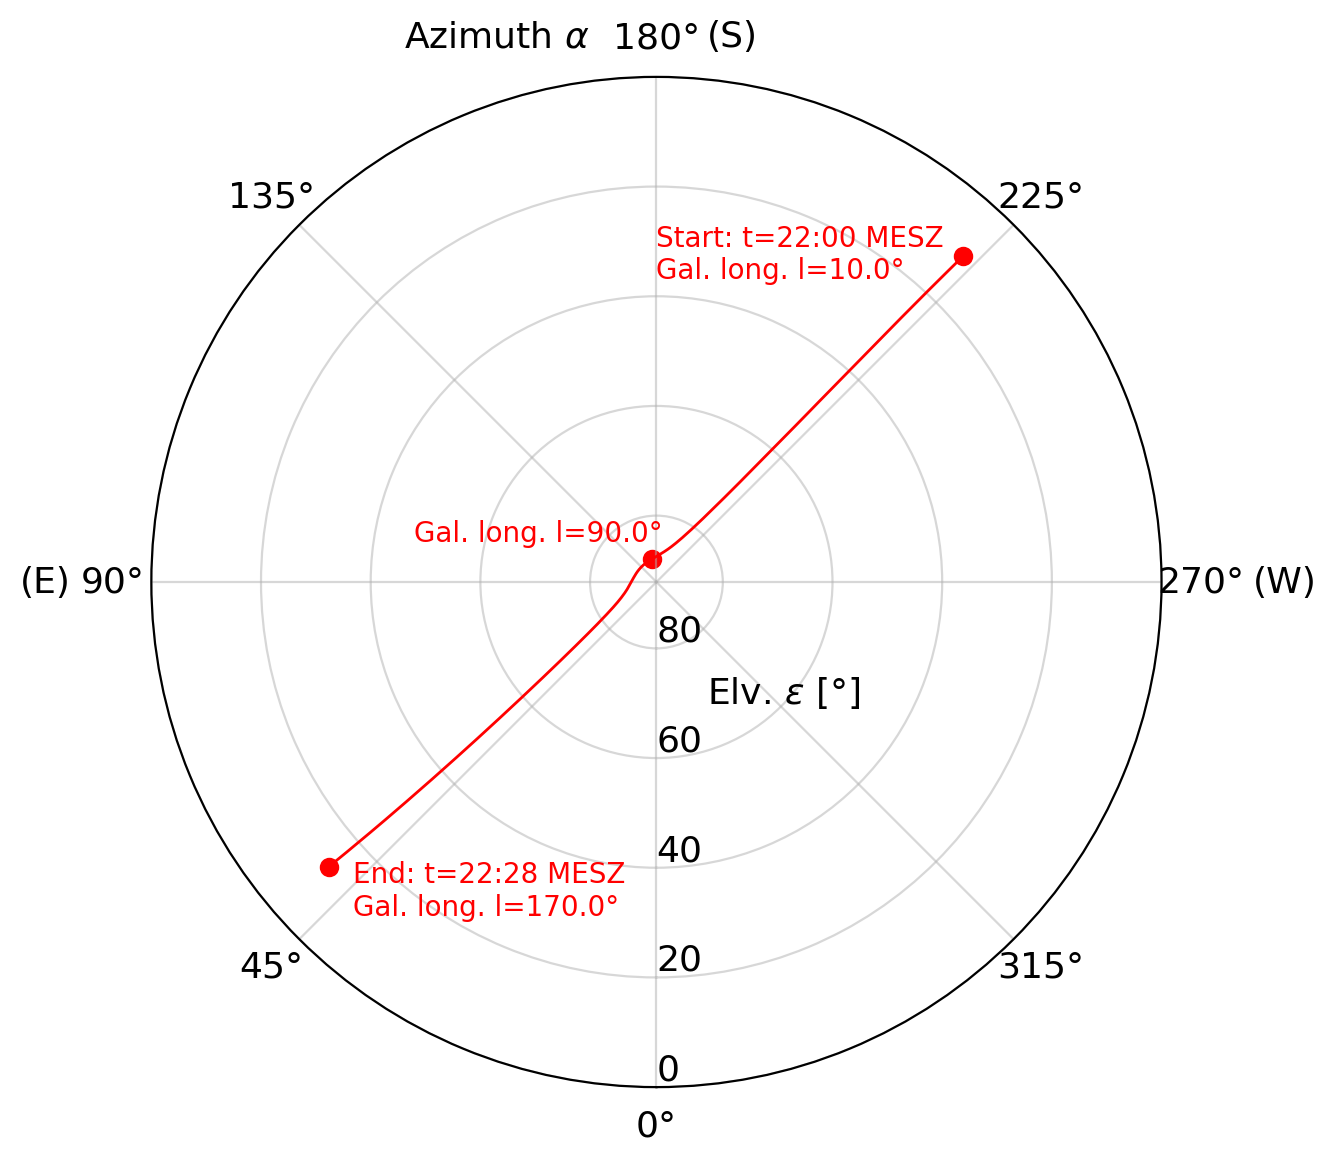
\includegraphics[width=10cm]{assets/mw_scan_polar.png}
    \caption{Polar plot of the Milky Way scan}
    \label{fig:mw_scan_polar}
\end{figure}

Figure \ref{fig:mw_spectrum_plot} shows the received power spectrum of the Milky Way scan. Vertically centred is the carrier frequency $f_c$ of the spectrometer, that matches the 21 cm wavelength of neutral oxygen ($f_c=$\SI{1420.4}{\giga\hertz}).
The brighter regions where more power was received show the emission from the hydrogen clouds in the Milky Way disc. A positive relative velocity $v_r>0$ between the earth and the emitting cloud result in a red shift and the maximal power received is shown in the lower half of the plot. For $v_r<0$ it is blue-shifted in the upper half. Some interesting regions are marked in red and will be discussed later.


\begin{figure}[H]
    \centering
    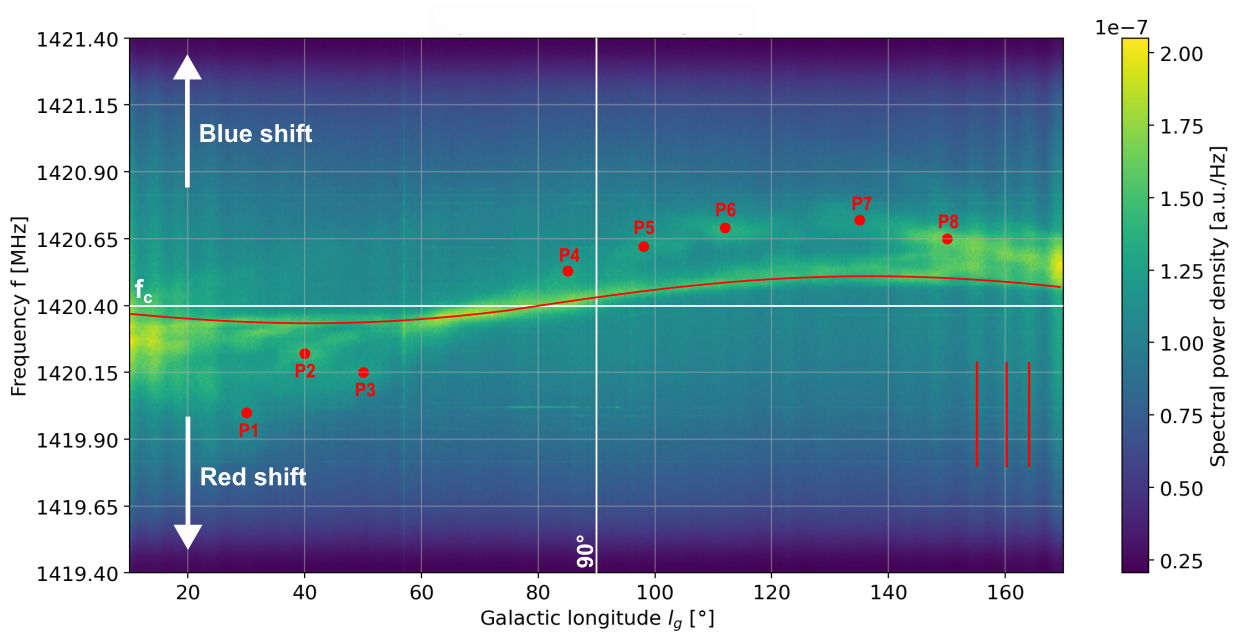
\includegraphics[width=\textwidth]{assets/spectrum_plot_edit.png}
    \caption{Received spectral power density vs. galactic longitude @ at zero latitude (galactic plane)}
    \label{fig:mw_spectrum_plot}
\end{figure}

We can identify following features in the spectrum plot:

\begin{itemize}
    \item The received spectrum from the hydrogen clouds is clearly red-shifted at longitudes below ~70° and blue shifted above. This was expected according explanation in section XXXXXX.
    \item The highest power density received, follow a sine shaped trend line (marked red). Most likely, this is the emission from the Perseus spiral arm of the Milky Way (Refer section \ref{sec:HotSpots}).
    \item There are some interesting regions with high radiation visible. Some of them are marked with Points P1 to P8 and will be discussed in section XXXXXX.
    \item We see some vertical lines of higher power density at low elevations (some marked red). These are caused from the high ground radiation that is amplified in the side lobes of the antenna characteristic as explained in section YYYYYY.
\end{itemize}



\subsubsection{Additional Exercise: Source determination of the hot spots}\label{sec:HotSpots}
In the Milky Way scan plot (figure \ref{fig:mw_spectrum_plot}) we have marked some hot spots of higher radiation. We tried to determine the sources of these spots in the Milky Way galactic disc. We have marked just spots with high red-/blue-shifts since a low shift results in very high inaccuracy in further calculations. \\
 \\
As explained in section ZZZZZ, we get the relation from the relative velocity $v_r$ to the radius $R$ of a radiating object in the galaxy plane in function of the galactic longitude $l_g$ using equation (XXXXXX). We considered the radial velocity as constant $v = v_0$ for all radii $R > 3kpc$, what is true for our positions we discuss. We can transform equation (XXXXX) to get the radius (in units of distance sun$\leftrightarrow$galactic center $R_0$) in function of the relative velocity and the galactic longitude as:

\begin{equation}
	\frac{R}{R_0}=\frac{v_0\cdot \sin(l_g)}{v_0\cdot \sin(l_g)-v_r}
\end{equation}

We can directly get $v_r$ from the Doppler shift. As $v_r$ is positive for red-shift, it is calculated as:

\begin{equation}
	v_r = \frac{f_c-f}{f_c} c
\end{equation}

From the hot spots marked in figure \ref{fig:mw_spectrum_plot}, we calculated the radii where the radiating source must be located. Finally, the position of the source is the intersection of the circle with the viewing line from the sun along the corresponding galactic longitude. We solved this problem graphically and drew the solution directly into the view of the Milky Way. In case of two solutions, we just marked the one closer to the sun. We did no error considerations for this task but we expect large uncertainties for the positions. Especially the red-shift caused by the orbital velocity of the earth around the sun (what is up to 30 km/s) is not considered and might result in a larger error. For the radii for P1...P8 in figure \ref{fig:mw_spectrum_plot}, we got...

\begin{table}[H]
\centering \footnotesize
\begin{tabular}{l r  r  r  r }
    \toprule
    Point & $l_g$ & $f$ [MHz] & $v_r$ [km/s] & $R/R_0$\\
    \midrule
    P1    &  30°  & 1420.00   &  84          & 0.57 \\
    P2    &  40°  & 1420.22   &  38          & 0.79 \\
    P3    &  50°  & 1420.15   &  53          & 0.76 \\
    P4    &  85°  & 1420.53   & -27          & 1.14 \\
    P5    &  98°  & 1420.62   & -46          & 1.27 \\
    P6    & 112°  & 1420.69   & -61          & 1.43 \\
    P7    & 135°  & 1420.72   & -68          & 1.77 \\
    P8    & 150°  & 1420.65   & -53          & 1.92 \\
    \bottomrule
\end{tabular}
\caption{Calculated relative velocities and red-/blue-shifts for points P1...P8.}
\label{tab:hot_spots}
\end{table}

... using $c=300'000$ km/s, $v_0 = 220$ km/s and $f_c=1420.4$ MHz.

\pagebreak

According $l_g$ and $R/R_0$ from table \ref{tab:hot_spots}, we evaluated the source positions for the points P1...P8 as shown in figure \ref{fig:mw_roi_spots}:

\begin{figure}[H]
    \centering
    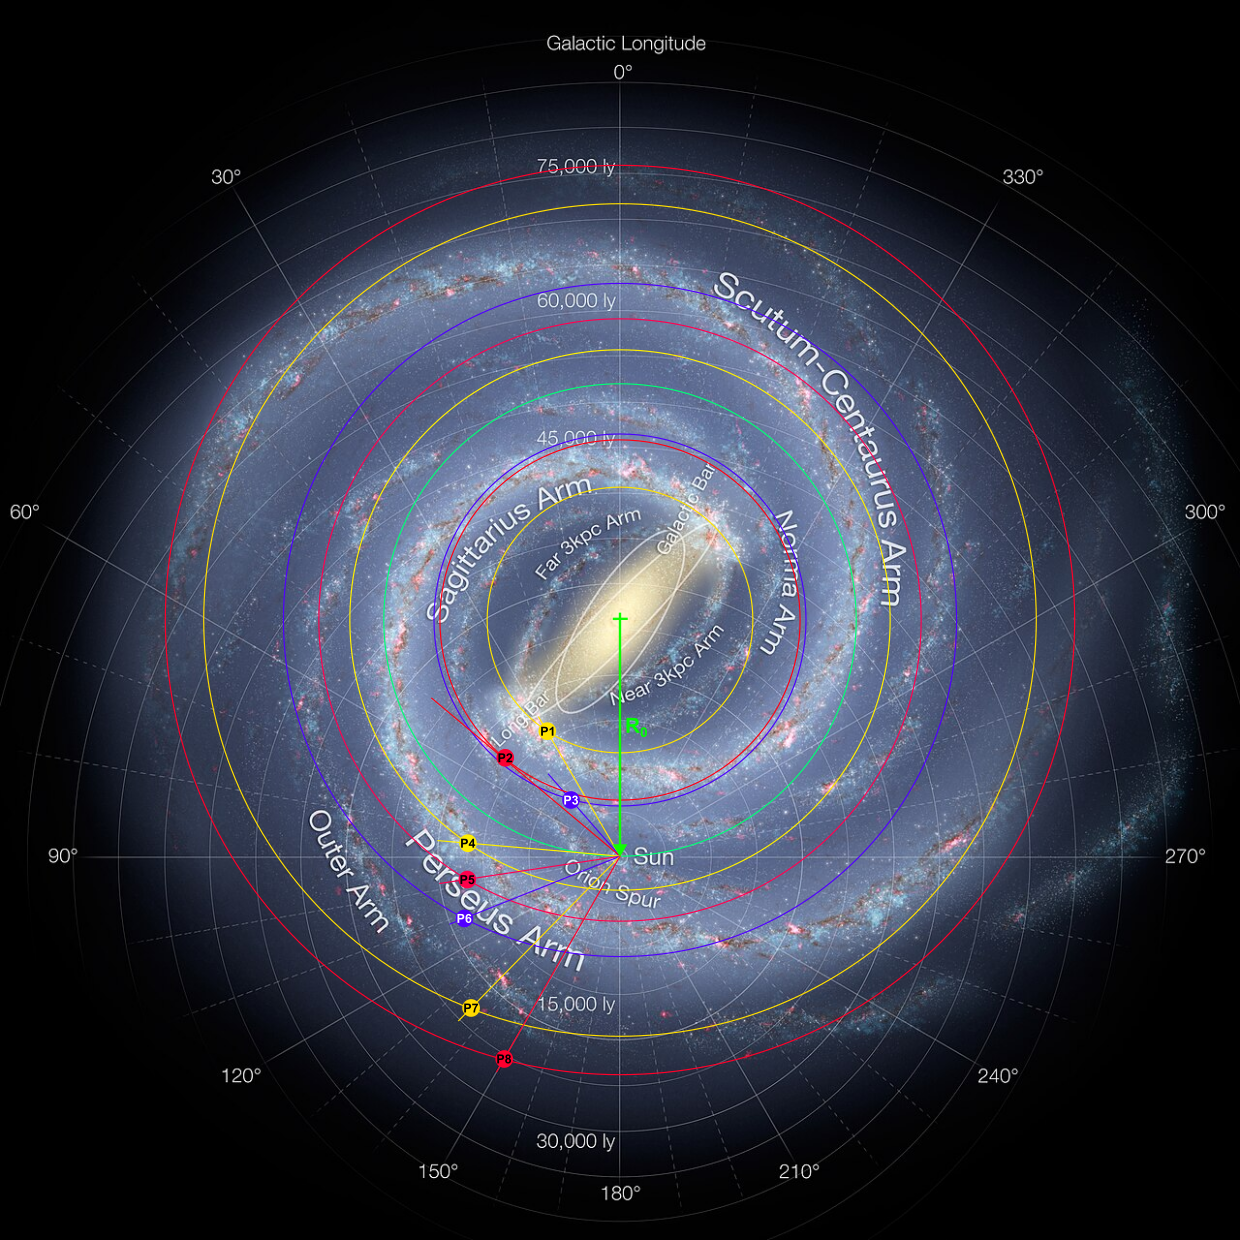
\includegraphics[width=\textwidth]{assets/MW_ROI_spots.png}
    \caption{Bla, Referenz XXXXXX}
    \label{fig:mw_roi_spots}
\end{figure}

We can see that most points are located in spiral arms with mutch higher concentrations of hydrogen. We suppose the sources for the hot spots in the spectrum plot are:
\begin{itemize}
	\item P1: Inner end of Scutum-Centaurs arm, at the near end of the long bar.
	\item P2, P3: Sources located in the Saggitarius arm
	\item P4, P5, P6: Sources located in the Perseus arm
	\item P7, P8: Not sure, maybe locations in the outer arm.
\end{itemize}

\pagebreak

\subsubsection{Additional Exercise: 2D-Scan of the Milky Way}\label{sec:MW_2D}
As additional exercise, we tried to perform a 2-dimensional scan of the Milky Way at the 07.10.2025. The idea was to do a scan the Milk Way along the galactic longitude of +10° to +160° with a latitude offset of -30°...+30°, what should be possible after 22:00 MESZ in the night. Unfortunately, we ran in several problems when using the Lab View tool. When the scan passes the zenith, the Lab View tool seems to have problem with the coordinate transformation. Therefore, we had to cut the record of the first scan at galactic longitude of 100° (close to the zenith at this time). To get more data in higher galactic longitudes, we tried a second scan at the 08.10.2025, 03:00 MESZ. This full scan was corrupt, as the SRT did not move, even if the galactic coordinates were correctly counting in the record. 24 hours later, we repeated the second scan successfully (Galactic longitude range: 160°...230°). Figure \ref{fig:mw_2d_polar} shows the scan lines of scan 1 and 2. The corrupted part of scan 1 (100°...160°) is marked red. The scan step size was 2.5° in both directions.

\begin{figure}[H]
    \centering
    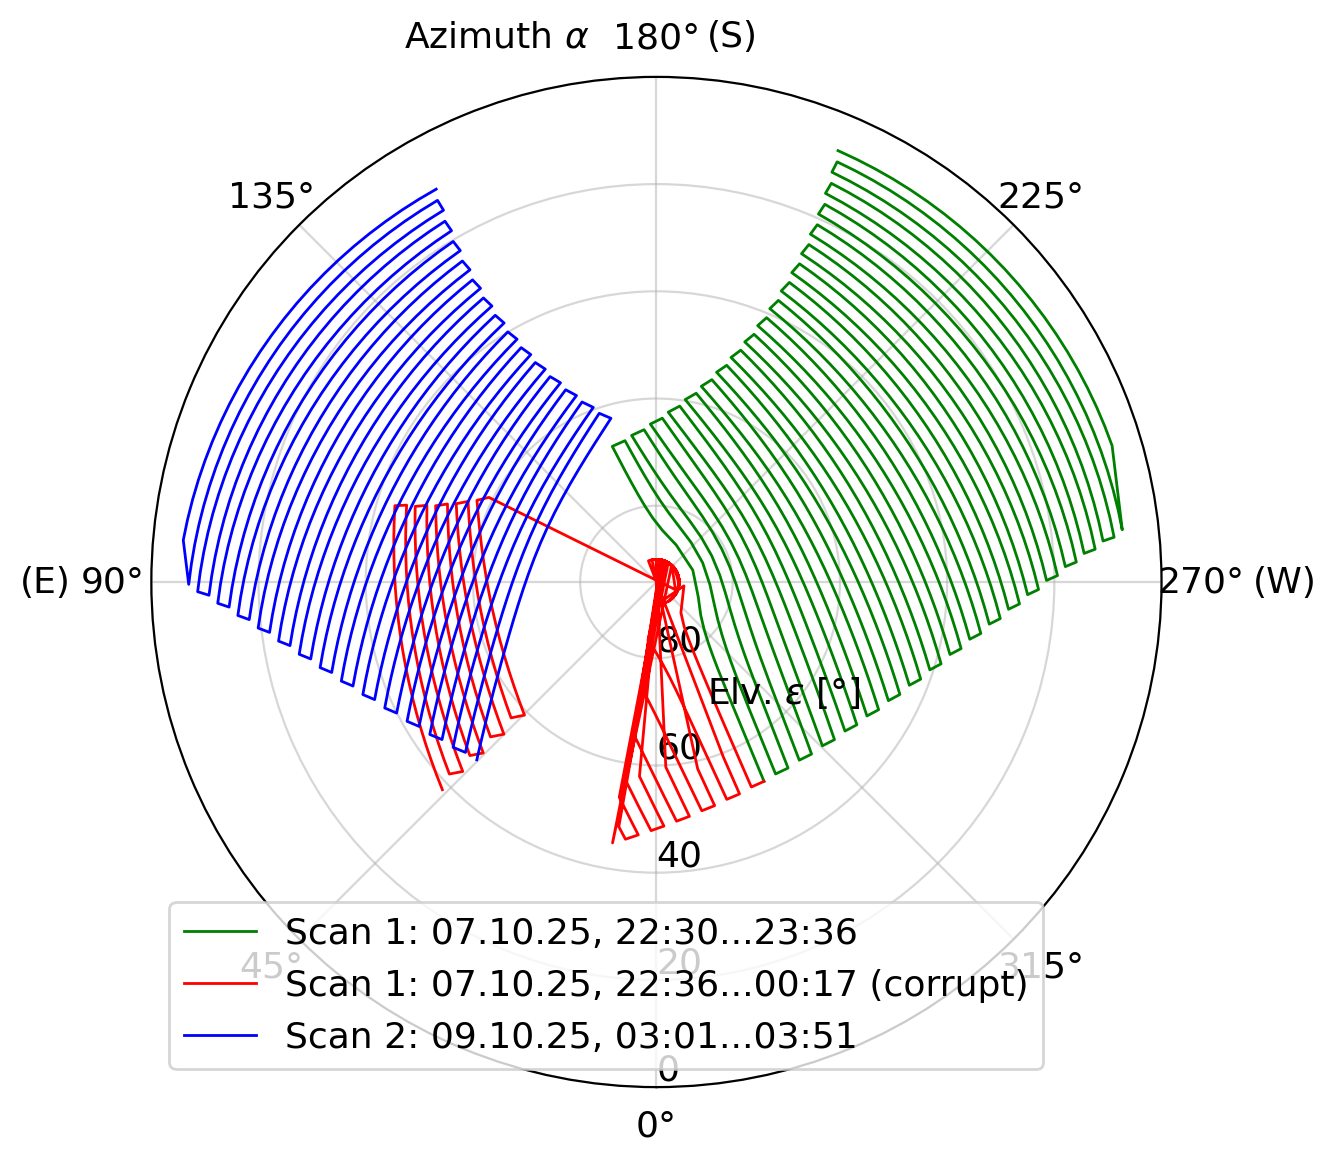
\includegraphics[width=12cm]{assets/mw2d_polar_plot.png}
    \caption{Polar plot of the Milky Way 2D scan paths}
    \label{fig:mw_2d_polar}
\end{figure}

We were not able to take a new scan of the corrupted section (100°...160° galactic longitude), without the scan passes the zenith or passes the azimuthal restrictions of the SRT. So we kept the corrupted section of the first scan and concatenated the two scans to get the full range of 10° to 230° galactic longitude in a 2-dimensional color plot as shown in figure \ref{fig:mw_2d_plot}. The corrupted section is marked.

\pagebreak

\begin{figure}[H]
    \centering
    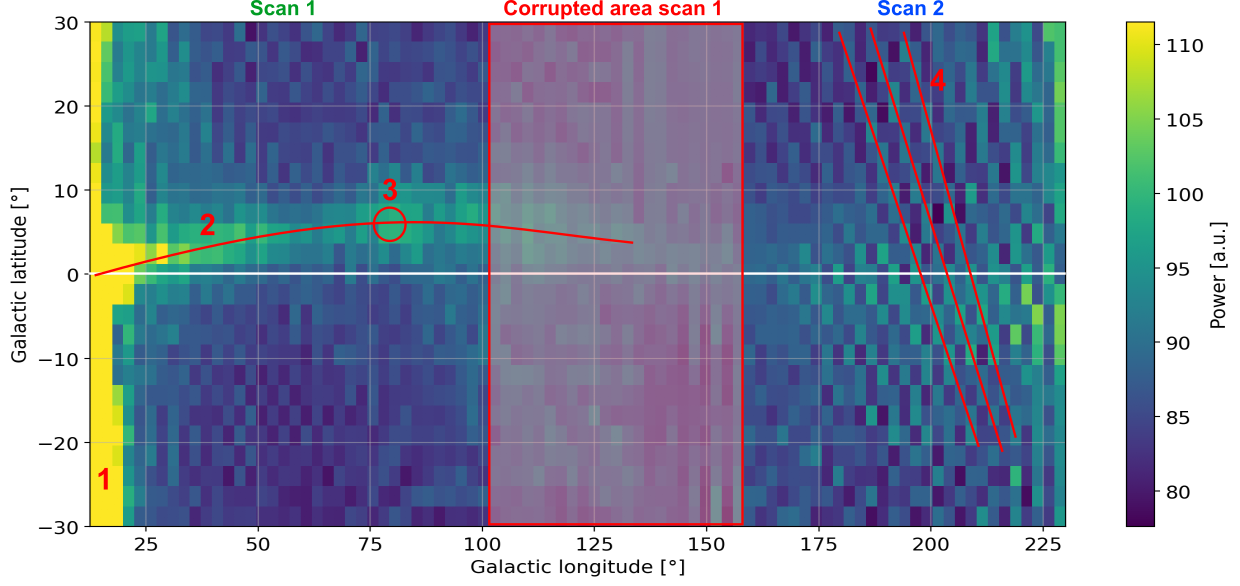
\includegraphics[width=\textwidth]{assets/mw2d_powermap_edit.png}
    \caption{Milky Way 2D scan: Galactiv coordinates vs. received power.}
    \label{fig:mw_2d_plot}
\end{figure}

We marked some features in the plot to discuss:
\begin{enumerate}
	\item The yellow region is the roof of the main building of the University of Bern. The higher power in this region was cut at the maximum power level of the remaining plot to get a better scale.
	\item We see a trend of the highest emissions in the galactic disc which are in a positive latitude of $\approx$ +5° around the longitude $\approx$ +90°. We find the same trend in the sky survey HI4PI [XXXXX].
	\item There is a bright region at galactic long./lat. $\approx$ +80°/+5°. This is possibly the galaxy Cygnus A, that is one of the brightest radio sources in the sky. Its center is located at +76°11'/+5°45' (RA/DEC J2000: 19h59m/40°44m), but the galaxy emits over a wider field, as shown in the paper \textit{Important Celestial Radio Sources} [YYYYY].
	\item The second scan seems somehow corrupted as well. First, we thought the power data was shifted somehow in the map. But, we did a check by applying exactly the same array reshape operations of the recorded data to the galactic coordinates and we found that the galactic coordinates that belongs to the power values are represented correctly in the 2-dimensional color plot (Refer to the data evaluation milky-way.ipynb). Further reasons for the pattern we see could be:
	\begin{itemize}
		\item There is still an undetected error in our data evaluation.
		\item There is a bright source on the ground (outside this plot) and we see its diffraction pattern (red lines).
		\item There was again a malfunction of the Lab View tool and the recorded power spectra do not belong to the represented. galactic coordinates.
	\end{itemize}
\end{enumerate}



XXXXX: https://www.icrar.org/hi4pi/ \\
YYYYY: https://reeve.com/Documents/Articles%20Papers/Reeve_CelestialRadioSources.pdf
\section{Conclusion}
The va



\subsection{Feedback}
Optionally include personal reflections on what was fun, challenging, or
interesting during the internship.



% -- Bibliography
\printbibliography

\vspace*{\fill}
\section*{Selbstständigkeitserklärung}

{\selectlanguage{german}
\enquote{
Ich erkläre hiermit, dass ich diese Arbeit/diese Prüfung selbstständig verfasst/beantwortet habe, keine weiteren Personen mir dabei geholfen haben, keine unerlaubten Hilfsmittel verwendet habe, und keine anderen als die angegebenen Quellen benutzt habe. Alle Stellen, die wörtlich oder sinngemäss aus Quellen entnommen wurden, habe ich als solche gekennzeichnet. Mir ist bekannt, dass andernfalls die Prüfung/die Arbeit mit der Note 1 bewertet wird bzw. der Senat gemäss Artikel 36 Absatz 1 Buchstabe r des Gesetzes vom 5. September 1996 über die Universität zum Entzug des auf Grund dieser Arbeit verliehenen Titels berechtigt ist.

Für die Zwecke der Begutachtung und der Überprüfung der Einhaltung der Selbständigkeitserklärung bzw. der Reglemente betreffend Plagiate erteile ich der Universität Bern das Recht, die dazu erforderlichen Personendaten zu bearbeiten und Nutzungshandlungen vorzunehmen, insbesondere die schriftliche Arbeit zu vervielfältigen und dauerhaft in einer Datenbank zu speichern sowie diese zur Überprüfung von Arbeiten Dritter zu verwenden oder hierzu zur Verfügung zu stellen.
}

\vspace{4cm}
\begin{tabular}{p{7.5cm}p{7.5cm}}
\hrulefill & \hrulefill \\
  Cedric Sigrist   &  Stefan Iseli
\end{tabular}
}

\end{document}